%%
%% Copyright 2007, 2008, 2009 Elsevier Ltd
%%
%% This file is part of the 'Elsarticle Bundle'.
%% ---------------------------------------------
%%
%% It may be distributed under the conditions of the LaTeX Project Public
%% License, either version 1.2 of this license or (at your option) any
%% later version.  The latest version of this license is in
%%    http://www.latex-project.org/lppl.txt
%% and version 1.2 or later is part of all distributions of LaTeX
%% version 1999/12/01 or later.
%%
%% The list of all files belonging to the 'Elsarticle Bundle' is
%% given in the file `manifest.txt'.
%%

%% Template article for Elsevier's document class `elsarticle'
%% with numbered style bibliographic references
%% SP 2008/03/01
%%
%%
%%
%% $Id: elsarticle-template-num.tex 4 2009-10-24 08:22:58Z rishi $
%%
%%
%%\documentclass[preprint,12pt]{elsarticle}
%%\documentclass[final,3p,times,twocolumn]{elsarticle}
\documentclass[final,3p,times,twocolumn]{elsarticle}

%% Use the option review to obtain double line spacing
%% \documentclass[preprint,review,12pt]{elsarticle}

%% Use the options 1p,twocolumn; 3p; 3p,twocolumn; 5p; or 5p,twocolumn
%% for a journal layout:
%% \documentclass[final,1p,times]{elsarticle}
%% \documentclass[final,1p,times,twocolumn]{elsarticle}
%% \documentclass[final,3p,times]{elsarticle}
%% \documentclass[final,3p,times,twocolumn]{elsarticle}
%% \documentclass[final,5p,times]{elsarticle}
%% \documentclass[final,5p,times,twocolumn]{elsarticle}

%% if you use PostScript figures in your article
%% use the graphics package for simple commands
%% \usepackage{graphics}
%% or use the graphicx package for more complicated commands
%% \usepackage{graphicx}
%% or use the epsfig package if you prefer to use the old commands
%% \usepackage{epsfig}

%% The amssymb package provides various useful mathematical symbols
\usepackage{amssymb}
%% The amsthm package provides extended theorem environments
%% \usepackage{amsthm}

%% The lineno packages adds line numbers. Start line numbering with
%% \begin{linenumbers}, end it with \end{linenumbers}. Or switch it on
%% for the whole article with \linenumbers after \end{frontmatter}.
%% \usepackage{lineno}

%% natbib.sty is loaded by default. However, natbib options can be
%% provided with \biboptions{...} command. Following options are
%% valid:

%%   round  -  round parentheses are used (default)
%%   square -  square brackets are used   [option]
%%   curly  -  curly braces are used      {option}
%%   angle  -  angle brackets are used    <option>
%%   semicolon  -  multiple citations separated by semi-colon
%%   colon  - same as semicolon, an earlier confusion
%%   comma  -  separated by comma
%%   numbers-  selects numerical citations
%%   super  -  numerical citations as superscripts
%%   sort   -  sorts multiple citations according to order in ref. list
%%   sort&compress   -  like sort, but also compresses numerical citations
%%   compress - compresses without sorting
%%
%% \biboptions{comma,round}

% \biboptions{}


\journal{NIMA}

\begin{document}

\begin{frontmatter}

%% Title, authors and addresses

%% use the tnoteref command within \title for footnotes;
%% use the tnotetext command for the associated footnote;
%% use the fnref command within \author or \address for footnotes;
%% use the fntext command for the associated footnote;
%% use the corref command within \author for corresponding author footnotes;
%% use the cortext command for the associated footnote;
%% use the ead command for the email address,
%% and the form \ead[url] for the home page:
%%
%% \title{Title\tnoteref{label1}}
%% \tnotetext[label1]{}
%% \author{Name\corref{cor1}\fnref{label2}}
%% \ead{email address}
%% \ead[url]{home page}
%% \fntext[label2]{}
%% \cortext[cor1]{}
%% \address{Address\fnref{label3}}
%% \fntext[label3]{}

\title{Performance of a 250L liquid Argon TPC
for sub-Gev charged particle identification}

%% use optional labels to link authors explicitly to addresses:
%% \author[label1,label2]{<author name>}
%% \address[label1]{<address>}
%% \address[label2]{<address>}

\author{J-PARC T32 collaboration}

\address{}

\begin{abstract}
%% Text of abstract

We have constructed a LArTPC detector with fiducial mass of ~150 kg
as a part of the R\&D program of the next generation neutrino and nucleon
decay detector.

This paper describes a study of particle identification performance of
the detector using well-defined charged particles
(pions, kaons, and protons) with momentum of ~800 MeV/$c$
obtained at J-PARC K1.1Br beamline.

\end{abstract}

\begin{keyword}
%% keywords here, in the form: keyword \sep keyword

%% MSC codes here, in the form: \MSC code \sep code
%% or \MSC[2008] code \sep code (2000 is the default)

\end{keyword}

\end{frontmatter}

%%
%% Start line numbering here if you want
%%
% \linenumbers

%% main text
%%%%%%%%%%%%%%%%%%%%%%%%%%%%%%%%%%%%%%%%%%%%%%%%%%
%\section{Introduction}
%%%%%%%%%%%%%%%%%%%%%%%%%%%%%%%%%%%%%%%%%%%%%%%%%%
%%%%%%%%%%%%%%%%%%%%%%%%%%%%%%%%%%%%%%%%%%%%%%%%%%
\section{Introduction}
%%%%%%%%%%%%%%%%%%%%%%%%%%%%%%%%%%%%%%%%%%%%%%%%%%
Refer \cite{Araoka:2011pw} for hardware/beam line description

%%%%%%%%%%%%%%%%%%%%%%%%%%%%%%%%%%%%%%%%%%%%%%%%%%
%\section{Detector Setup}
%%%%%%%%%%%%%%%%%%%%%%%%%%%%%%%%%%%%%%%%%%%%%%%%%%
\section{Experimental Setup}

We have described details of the experimental setup in ref.\cite{Araoka:2011pw},
and in this paper we only discuss the issues which are relevant.

\subsection{K1.1Br Beamline}
K1.1Br beamline is located at J-PARC slow extraction facility.
It is designed and constructed for TREK experiment~\cite{ref:TREK}. 
to obtain high intensity and high purity $K^+$ beam with momentum around 800 MeV/$c$.
30 GeV/$c$ protons are irradiated to production target, and bending magnets
and an electo-static separator (ESS) provide excelent momentum separation and mass separation, respectively.
Other than $K^+$, Protons and $\pi^+$ and $e^+$ are also available in this beamline. 
While October 2010 run period, using 3.6 kW of 30 GeV/$c$ proton on target, 
TREK collaboration have achieved $K/\pi$ ratio of $\sim$1 with Kaon rate of $\sim$1 kHz.
For LArTPC test, we have intentionally reduced the beam intensity to $\sim$ 10 Hz 
to avoid particle overwrap, and maximum achived  $K/\pi$ with this condition was $\sim$1/4.

800 Mev/$c$ $\pi^+$ and $K^+$ are passing-through the 250L TPC detector.
We reduce their momentum to $\sim$600 MeV/$c$ and $\sim$200 MeV/$c$, respetcively,
so that they stop inside the TPC fiducial volume.
200 MeV/$c$ $\pi^+$ is obtained by changing the beamline optics and turning off ESS,
because $\pi^+$(and $e^+$) is dominant component without ESS.
To obeain 600 MeV/$c$ $K^+$, a beam degrader is located at downstream of the beamline
and $K^+$ lose its enery by ionization.We use a combination of lead glass blocks (LG) 
and lead brick (LB) as beam degrader with thckness of 12.5 cm and 2.5 cm, respectively.

\subsection{250L Detector}

The cryostat..

The TPC we have build for this test is a simple grid chamber
with active volume of 40 cm$\times$ 40 cm$\times$ 76 cm$\times$.

Cathode plane and anode plane is located at 
at the bottom and top of the field cage, respectively,
and grid plane is inserted 1 cm from the anode plane.
Side of the TPC us surrounded by field shapers.

The cathode and grid planes are 100 $\mu$m stainless steel wire
spaced by 5 mm.

The Anode is made with PCB (printed circuit board) with readout pitch of 1 cm.
Substrate of PCB is 1.6 mm FR-4 glass-rainforced epoxy
and electrode is 100 $\mu$m of gold-plated copper.

The field shaper is also made with PCB


The charge

12 bit ADC with 2.5 MHz sampling frequency

\subsection{Beamline Equipment}

We have several beam counters to identify beam particles.
% (see Fig\ref{fig:Beamline}).
There are two beam defining counters (BDC and T32 BDC) which determine acceptance of the beam, 
a Fitch-type Cherenkov counter (FC), and a Gas Cherenkov counter (GC), 
and two time of flight counters (TOF1 and TOF2).

%\begin{figure}[htbp]
%  \centering
%  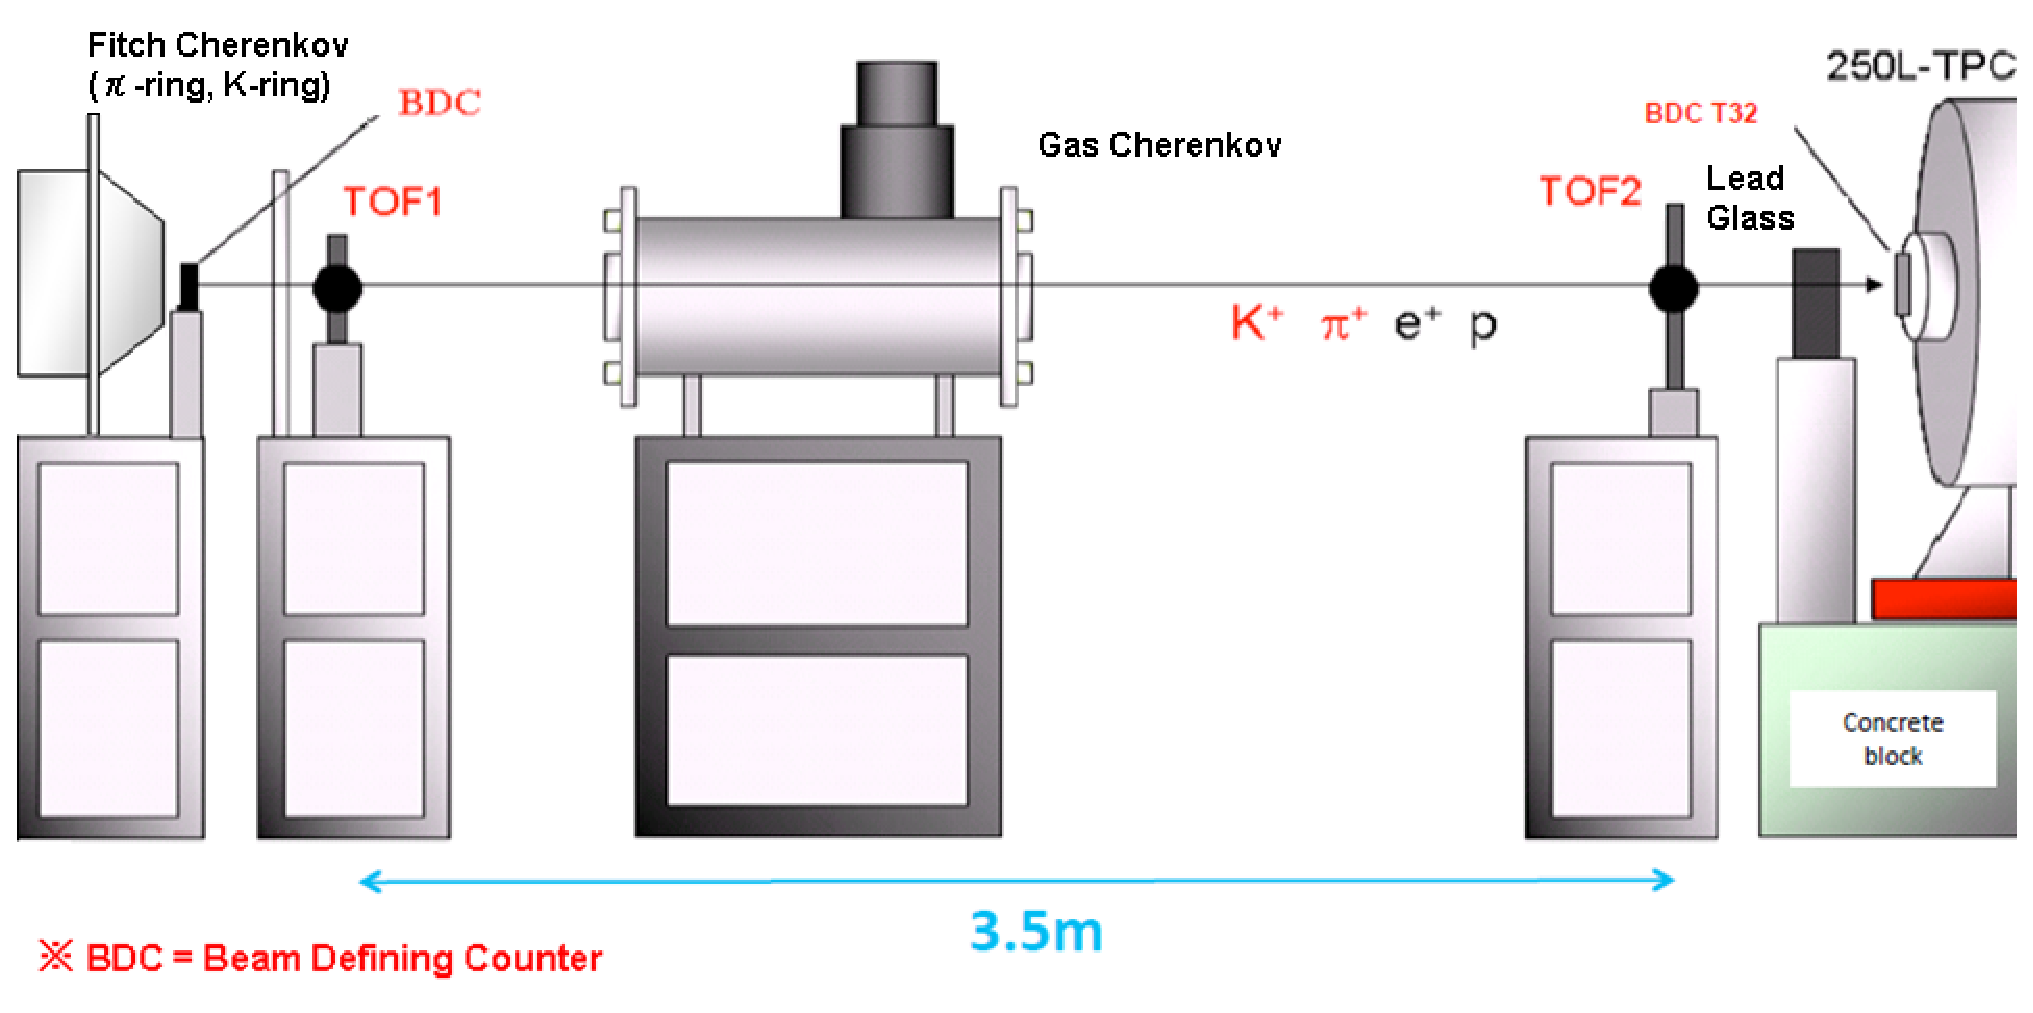
\includegraphics[width=1.0\hsize,clip]{fig/Beamline.eps}
%  \caption{Instruments on K1.1BR Beam Line}
%  \label{fig:Beamline}
%\end{figure}

Two TOF counters are about 3.5m apart, and time resolution is abot $\sim$200 ps.
Figure \ref{fig:BeamCountersTOF} shows the flight time distribution between TOF1 and TOF2
obtained from 800 MeV/$c$ beam particles which contain  $K^{+}$, $\pi{+}$, $e^{+}$, and $p$. 
Three peaks which correspond to $\pi$+$e^+$, $K^+$, and $p$, respectively, are well separated.
FC has 4 cm of acrylic plate as Cherenkov light radiator and 
photo-multipliers which are aligned in circles with two different emission angles
($K$-ring and $\pi$-ring) as photo detector. It is designed to have maximum separation of 
$K^{+}$ and $\pi^{+}$ with momentum of 800 MeV/$c$.
Top plot in Fig.\ref{fig:BeamCountersFC} shows response of FC for the 800 MeV/$c$ beam particles. 
Horizontal axis and vertical axis are hit multiplicity of the $\pi$-ring and $K$-ring, respectively. 
$K^+$($\pi$) is identified as event with signal in $K$-ring ($\pi$-ring) but no signal in $\pi$-ring ($K$-ring).
In case of no signals in both rings, the particle is considered as proton.
Additional separation between $e^{+}$ from $\pi^+$ is provided by GC 
which uses atmospheric air as Cherenkov radiator. 
Filled histograms in bottom plot of Fig.\ref{fig:BeamCounters} shows selected $K^+$ event with FC information.
After removing residual $\pi^+$ using TOF, $K^+$ sample is almost 100\% purity.

\begin{figure}[htbp]
  \begin{center}
    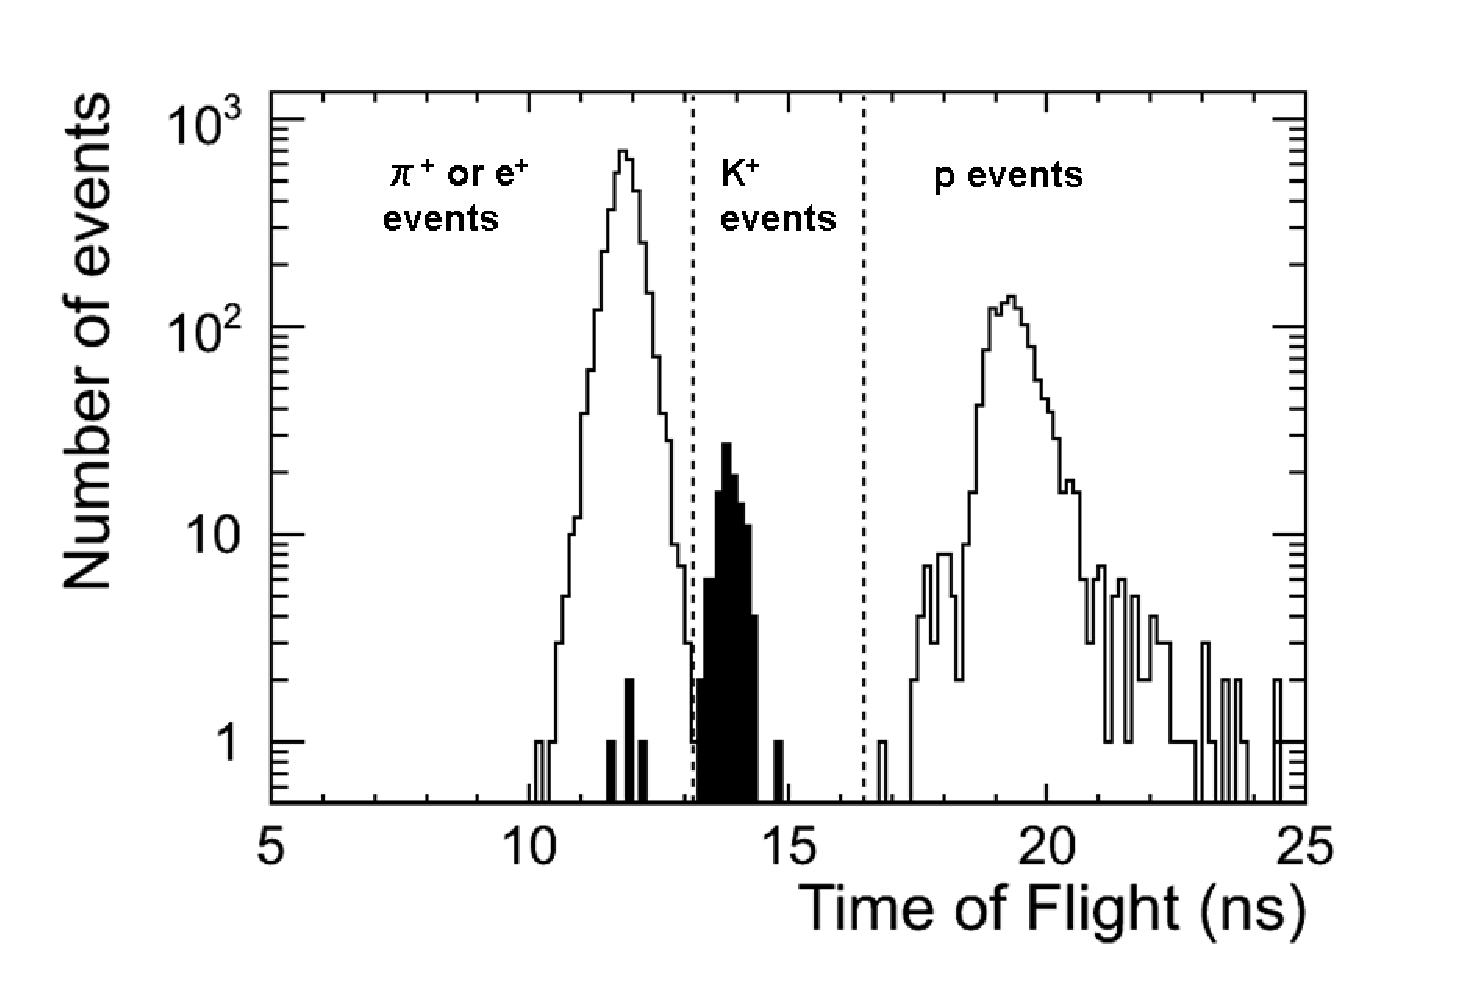
\includegraphics[width=1.0\hsize,clip]{fig/TOF_cut.eps}
  \end{center}
 \caption{TOF distribution.}
 \label{fig:BeamCountersTOF}
\end{figure}

\begin{figure}[htbp]
  \begin{center}
    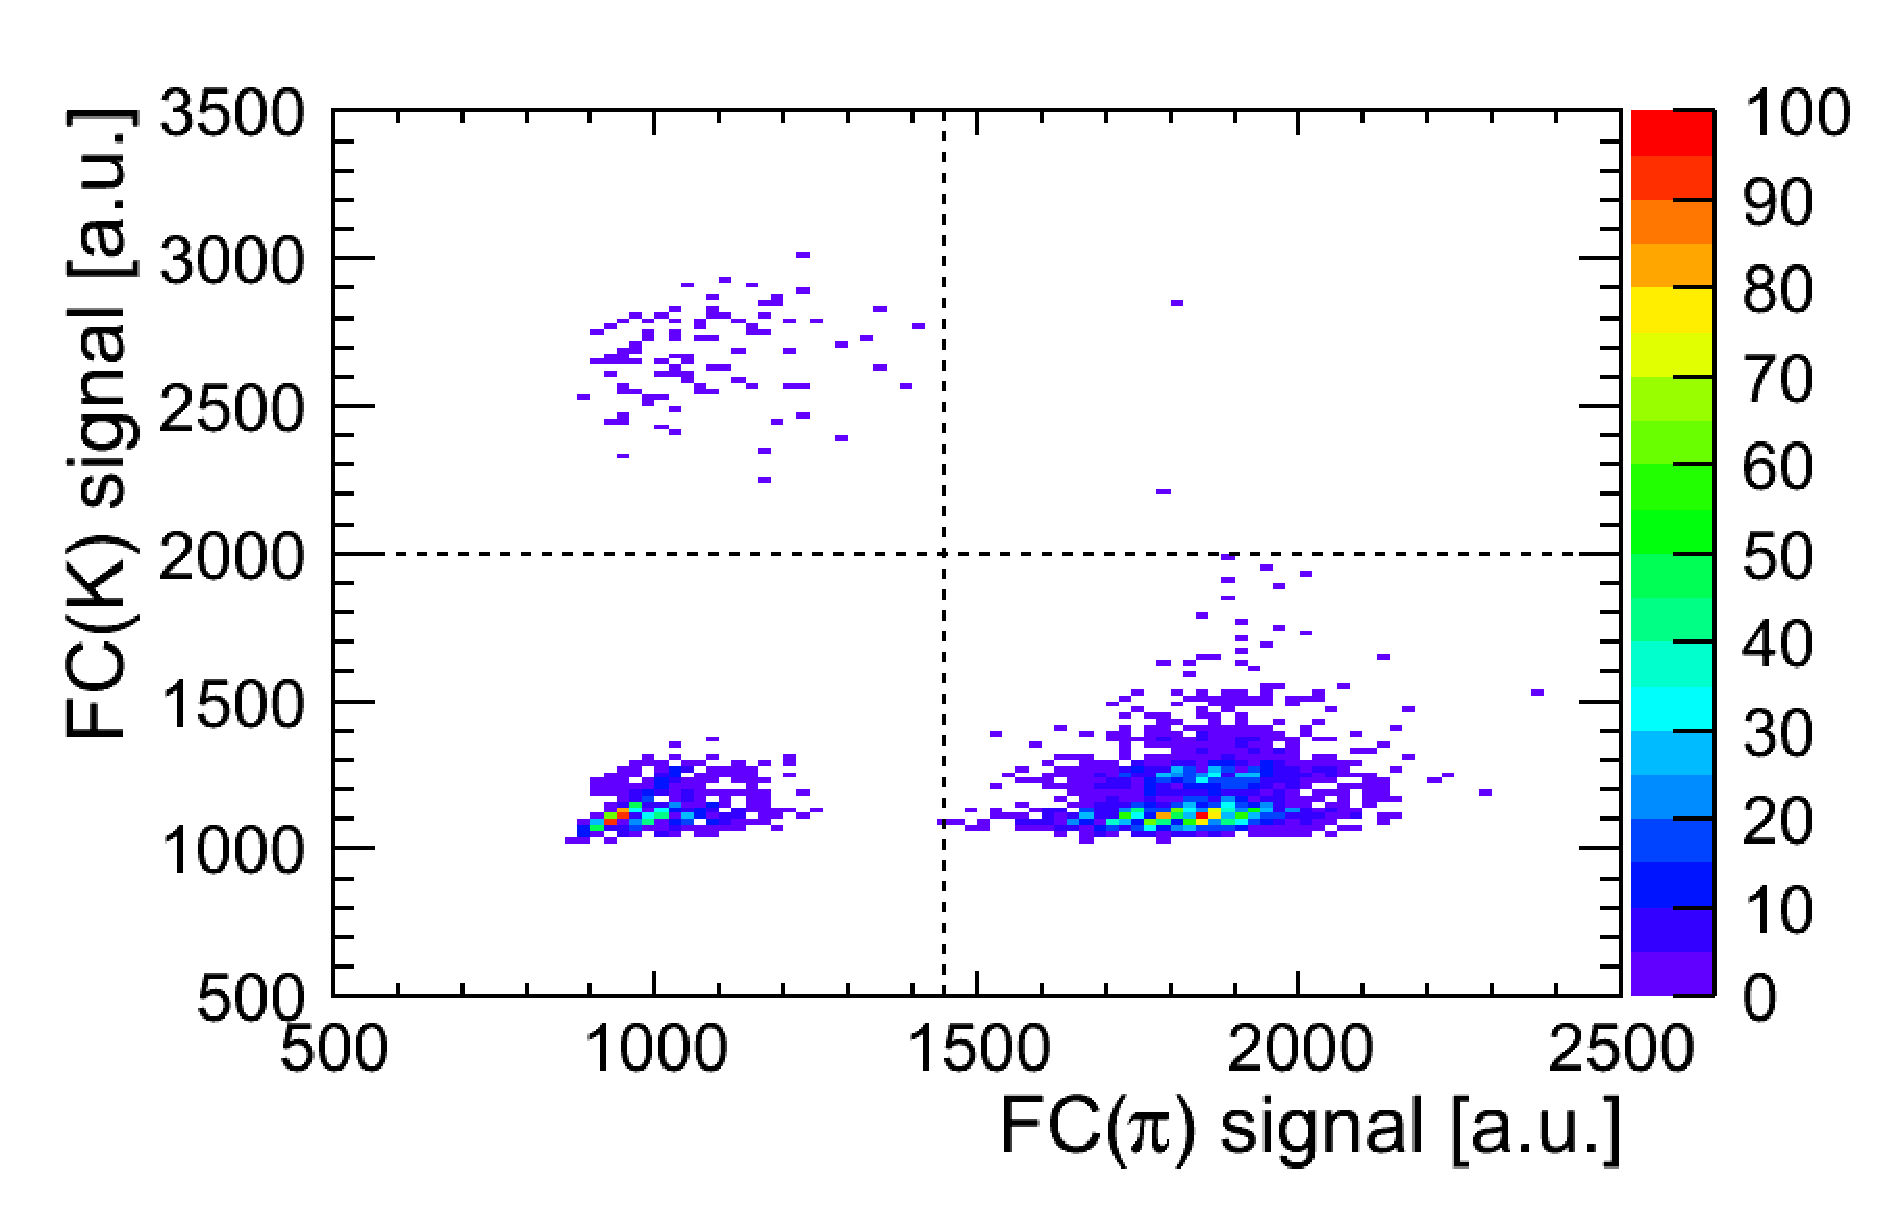
\includegraphics[width=1.0\hsize,clip]{fig/FC_KPI.eps}
  \end{center}
 \caption{FC}
 \label{fig:BeamCountersFC}
\end{figure}


\subsection{Oct/2010 Beam Test Configuration}

by using the beam counters, we define three types of triggers:
(i) non-bias trigger simply requires signal in two BDCs and two TOFs;
(ii) Kaon trigger requires, in addition to non-bias trigger, K identification with FC information;
(iii) electron trigger rquires, in addition to non-bias trigger, electron identification with GC information.

Beam Momentum
\begin{itemize}
\item Materials located from proton target to LArTPC detector (beam counters, beam windows, air, etc) degrade beam particle momentum
\item the effect is estimated by looking at TOF of proton, average prton beam momentum is 730 MeV/$c$
\item For other particles  (K, pi,e e), TOF does not have enough resolution to determin momentum, and the degradation
is directly estimated by counting the energy deposition to the materials using GEANT based simulation.
For example Kaon momentum is xxx MeV/c on average.
\end{itemize}

\begin{figure}[htbp]
  \begin{center}
    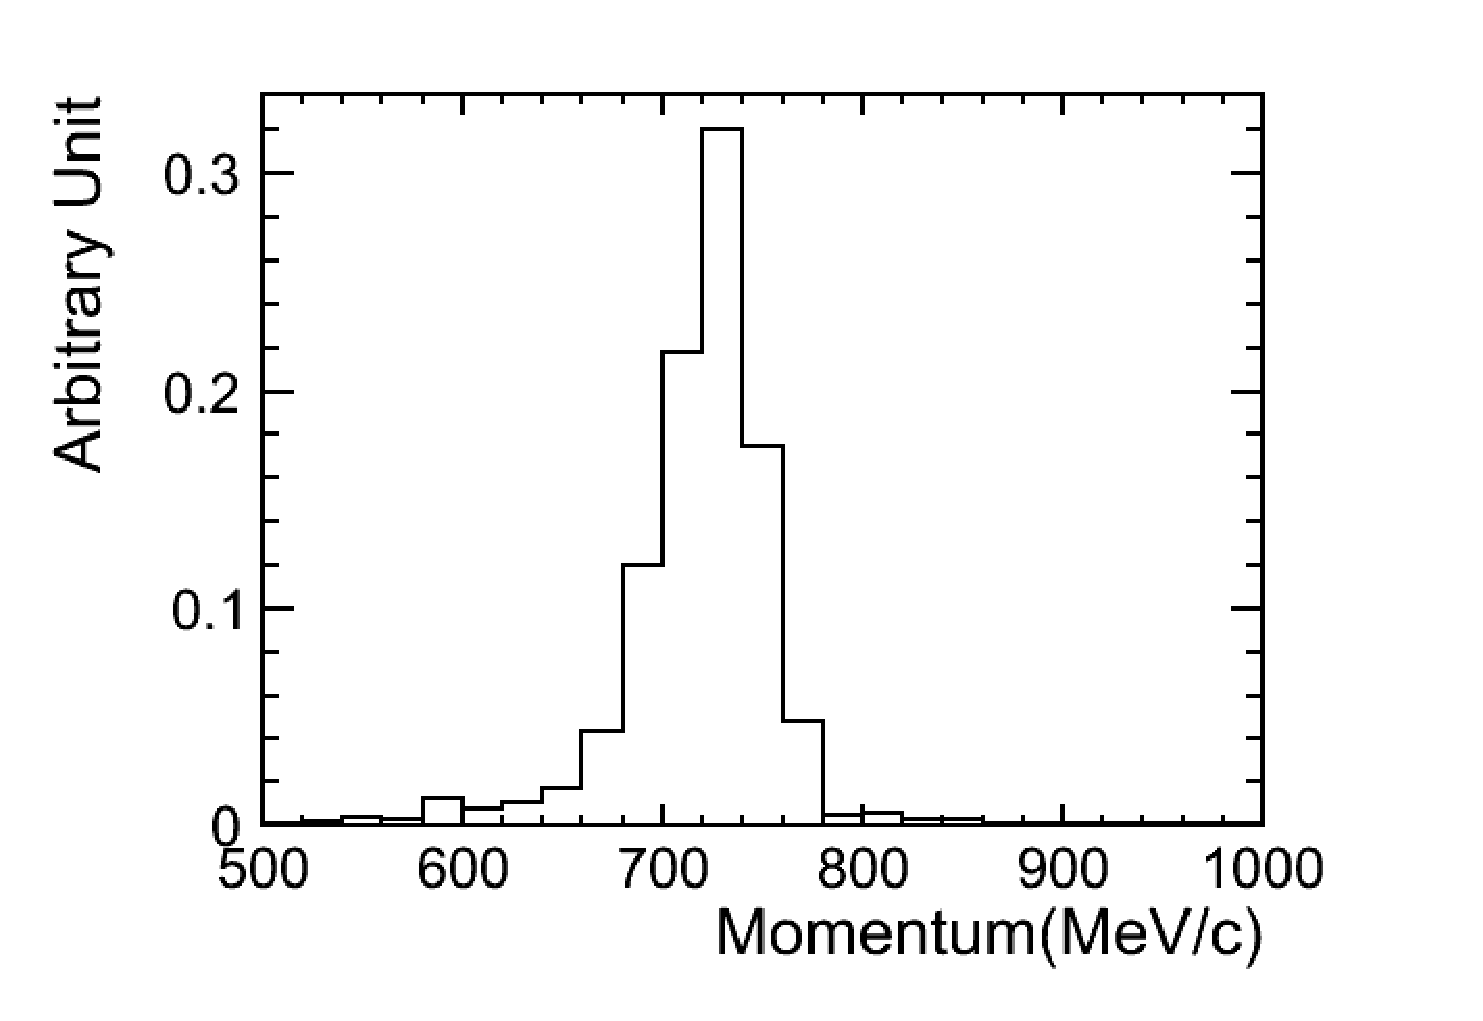
\includegraphics[width=1.0\hsize,clip]{fig/Momentum_proton.eps}
    \caption{Top plot shows $\rm {\Delta TOF}$ distribution of TOF counters with proton data,
      and bottom plot shows proton momentum estimated by $\rm {\Delta TOF}$ of TOF counters information}
    \label{fig:Proton_momentum}
  \end{center}
\end{figure} 

We measured beam profile in front of 250LAr TPC beam window by using plastic scintillation counters.
%Figure \ref{beamprofile_250L} shows the result.
The beam is relatively narrow in vertical direction (within 5 cm),
but spread in horizontal direction ($\sim$ 10 cm).

%\begin{figure}[!htb]
%  \begin{center}
%     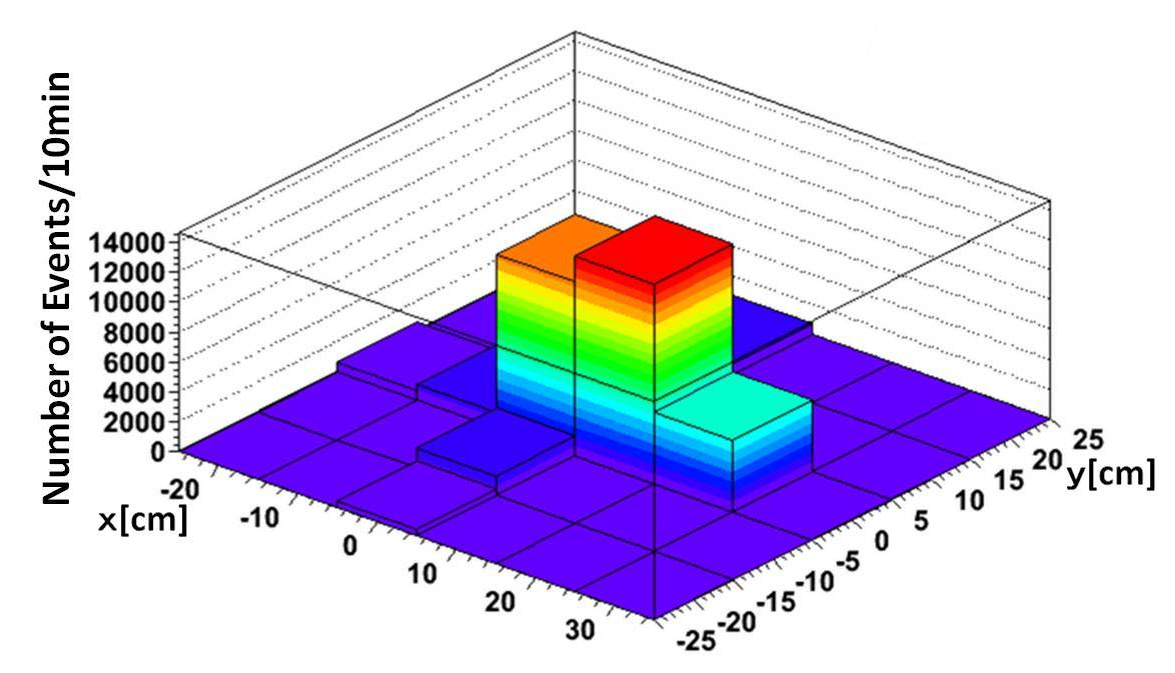
\includegraphics[width=0.8\hsize,clip]{./fig/BeamProfile3.eps}
%  \end{center}
%  \caption{Beam profile on the front of 250LAr TPC}
%  \label{beamprofile_250L}
%\end{figure}



%%%%%%%%%%%%%%%%%%%%%%%%%%%%%%%%%%%%%%%%%%%%%%%%%%
%\section{Data Sampple}
%%%%%%%%%%%%%%%%%%%%%%%%%%%%%%%%%%%%%%%%%%%%%%%%%%
%%%%%%%%%%%%%%%%%%%%%%%%%%%%%%%%%%%%%%%%%%%%%%%%%
\section{Data Sample}
%%%%%%%%%%%%%%%%%%%%%%%%%%%%%%%%%%%%%%%%%%%%%%%%%%
\subsection{Collected Data}
Table~\ref{Table:Data} shows list of the collected data while Oct/2010 Run.
800 MeV/$c$ $\pi^+$ is expected to pass-through the detector as almost minimum ionizing,
and have uniform energy deposition to all the TPC channels.
So this data set is useful for calibrating the detector response (See Sec.~\ref{Sec:Pion}).
800 MeV/$c$ proton stops after ~15 cm of flight distance inside the TPC fiducial volume
with relatively large $dE/dx$. So we use the proton data set for validation of the
detector response at high $dE/dx$ region(See Sec.~\ref{Sec:Proton}).
We have collected three different $K^+$ data by varying thickness of the degrader. 
540, 630, 680 MeV/$c$ correspond to the momentum degraded by 
2 lead glass, 1 lead glass + 1 lead block, and 1 lead glass, respectively, 
and such $K^+$ stops after 10 cm, 50 cm, and 65 cm of flight distance inside TPC fiducial volume.

\begin{table}[h]
\begin{center}
\caption{List of collected data}
\begin{tabular}{l|ll}
  Particle  &Momentum (MeV/$c$) &Number of Events\\
\hline
  Pion      &800                &3,000\\
  Proton    &800                &1,500\\
  Kaon      &540 (2LG)          &7,000\\
  Kaon      &630 (1LG+1LB)      &40,000\\
  Kaon      &680 (1LB)          &35,000\\
  electron  &800                &2,500\\
  electron  &200                &10,000\\
  pion      &200                &10,000\\
\end{tabular}
\label{Table:Data}
\end{center}
\end{table}

Top plot in Fig.~\ref{Fig:Textbook} shows 2D display of an event taken with 800 MeV/$c$ electron trigger.
Horizontal axis corresponds to TPC channel number where zero means most upper stream strip. 
Since strip pitch is 1 cm, this is equivalent to distance from beam injection point in cm.
Vertical axis corresponds to electron drift time in $\mu$s
where t=0 means trigger timing. 
In 250L TPC, anode and cathode is located at top and bottom of the detector, respectively,
drift direction is from bottom to top of the detector.
With 200 V/cm of electric field, drift velocity is about 0.8 m/ms,
and drift time of full detector (40 cm) is about 500 $\mu$s.
Color strength of the plot corresponds to the TPC signal pulse height in ADC counts.
In this event, triggered electron can be clearly identified in the center of the detector
as an electromagnetic shower,  while there are two other particles 
accidentally overlapped with the triggered electron. 
Track at t=100 $\mu$s is considered as
a proton which stops after 15 cm of flight distance and 
has large $dE/dx$ around the stopped point.
Track at t=400 $\mu$s is considered as
a pion which passes-through the detector and 
has uniform $dE/dx$ over the TPC channels.
Bottom plot in Fig.~\ref{Fig:Textbook} shows a typical $K^+ \to\mu^+\nu$ like event.
We can clearly identify a kink of the track at 60 cm which is considered
as stopped point of Kaon and it decays to $\mu^+\nu$ .
Energy deposition of the track is about MIP at the injection point
and gradually increase towards the stopped point at 60 cm.

\begin{figure}[htbp]
 \begin{center}
  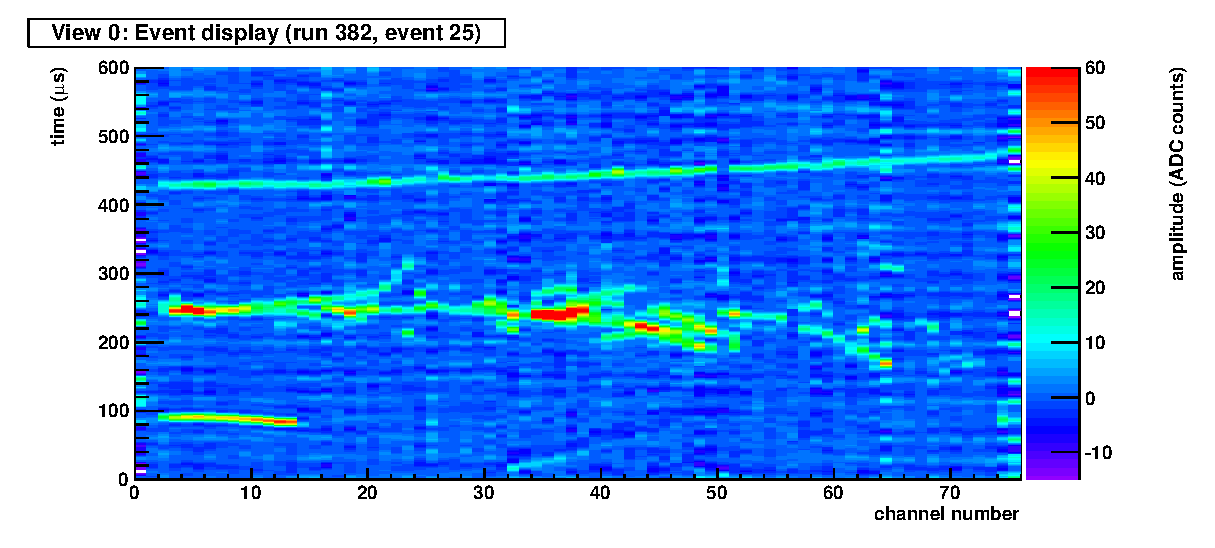
\includegraphics[width=1.0\hsize]{fig/Textbook.eps}
  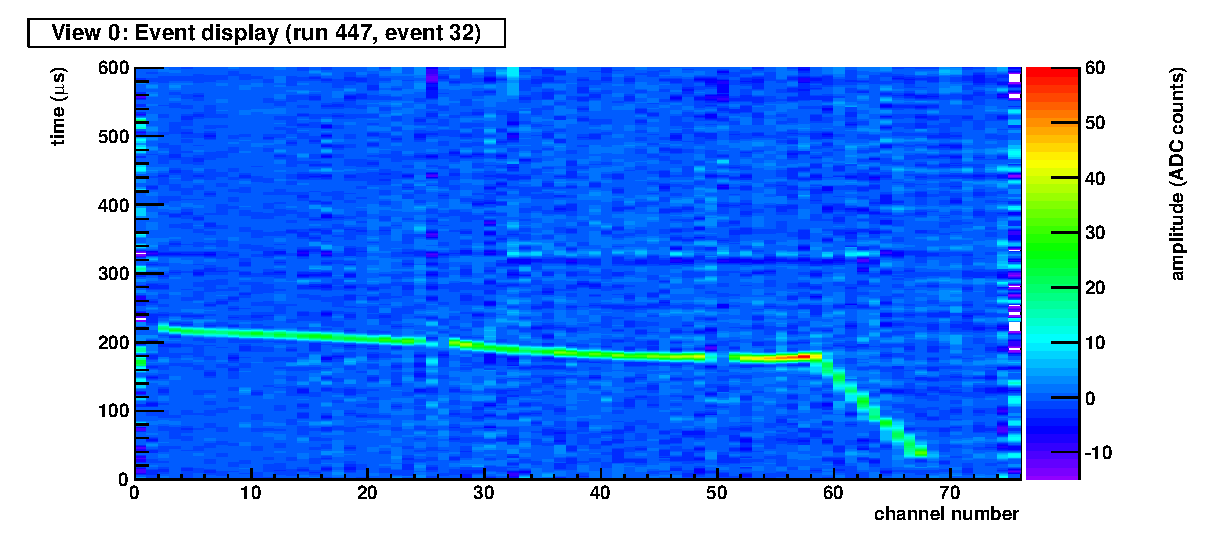
\includegraphics[width=1.0\hsize]{fig/Kmunu.eps}
 \end{center}
 \caption{Event display of 800 MeV/$c$ electron triggered event (top) accidentally overlapped with a proton and a pion,
   and Kaon 630 MeV/$c$ triggered event (bottom)}
 \label{Fig:Textbook}
\end{figure}


\subsubsection{Noise Reduction}
Dotted line in top plots of Fig.~\ref{Fig:FFT} shows raw waveform of the TPC signal
before applying any noise reduction. the waveform shown in this plot
are channel 13 in Fig.~\ref{Fig:Textbook} which are around the proton stopped point.
Signal-to-noise ratio for this particular case is poor and pion signal 
which is supposed to be t=400 $\mu$s is almost hidden by the noise. 
While time width of TPC signal is few $\mu$s which is determined by
drift time between anode and anode-grid, dominant noise component looks
higher frequency. To reduce such noises, we have applied FFT 
(Fast Flourier Transformation) filter to cut the high frequency component.
Bottom plot in Fig.~\ref{Fig:FFT} shows amplitude as a function of frequency
for the same event. This clearly shows dominant noise component with
$>$ 200 kHz has good separation with signal component ($<$ 100 kHz).
Solid line in top plot of Fig.~\ref{Fig:FFT} shows waveform after removing high frequency
($>$ 80 kHz) component by the FFT filter. Signal-to-noise ratio is dramatically
improved. On the other hand, we expect certain bias to the signal charge
measurement by this filter, and it will be discussed in Section x.

\begin{figure}[htbp]
 \begin{center}
  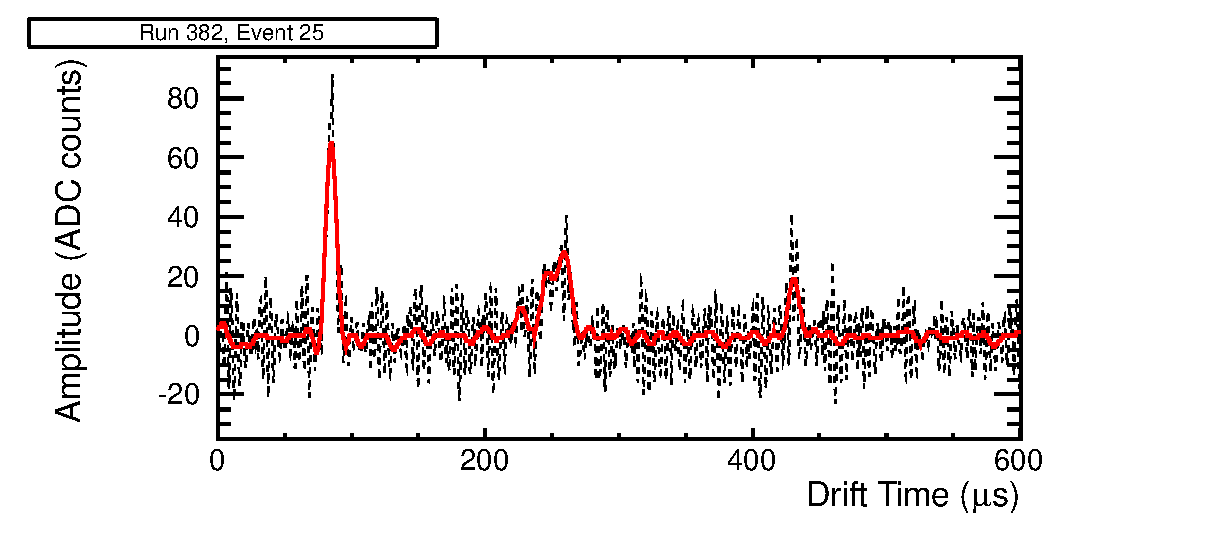
\includegraphics[width=1.0\hsize]{fig/beforeafterFFT.eps}
  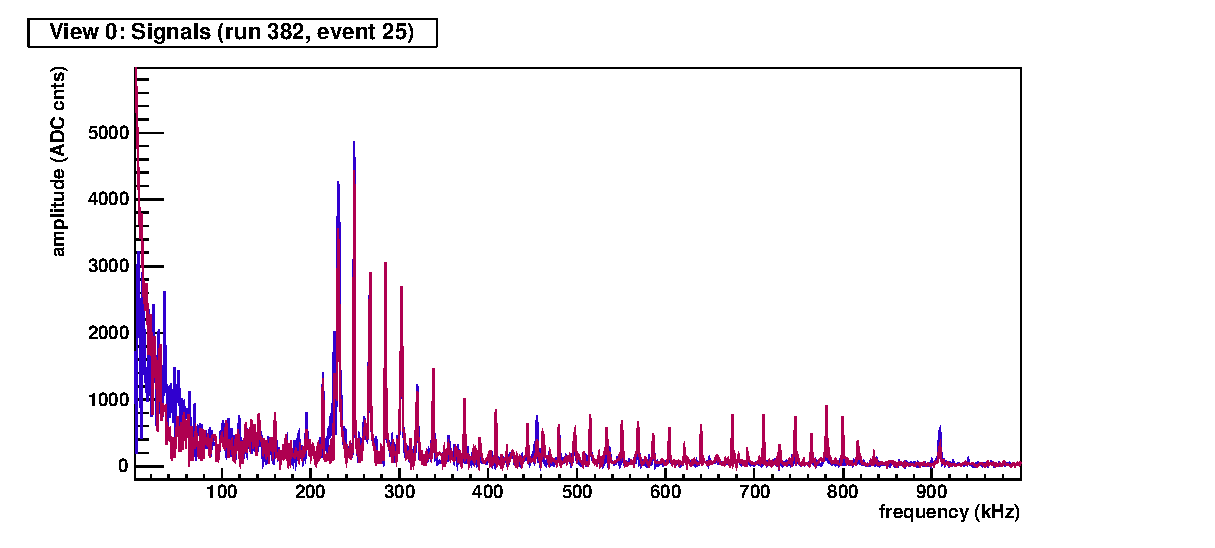
\includegraphics[width=1.0\hsize]{fig/FFT.eps}
 \end{center}
 \caption{Top: Typical TPC signal waveform before (dotted line) and after (solid line) applying FFT low pass filter with threshold of 80 kHz,
Bottom: FFT frequency amplitude distribution}
 \label{Fig:FFT}
\end{figure}


\subsubsection{Hit Finding/Clustering}
After noise reduction we find signal hits and create clusters associated to single tracks. 
Hit is defined as bump over given threshold in a channel. 
Threshold of hit finding is 6 ADC counts, which is about 2.5$\sigma$ from typical data noise level (as shown in Fig~\ref{Fig:FFT}) and keeping more than 99\% of Kaon hit finding efficiency in simulation.
% noise level from outside window of PhysicsOct55 (rms~2.49)
ADC count distribution is fitted by Gaussian plus step function to estimate the charge of hit in ADC $\times$ $\mu$s unit.
Fitting $\chi^2 < 3$ and $2.5<$~(time~width~of~hit)~$<8$~$\mu$s are required to remove noise hits further.
After finding all hits in an event, we construct cluster by merging adjacent hits. 
The example of hit finding and clustering using Fig~\ref{Fig:Textbook} event is shown in Fig~\ref{fig:Clustering}, which indicates reasonable hit and cluster findings. 

\begin{figure}[htbp]
 \begin{center}
  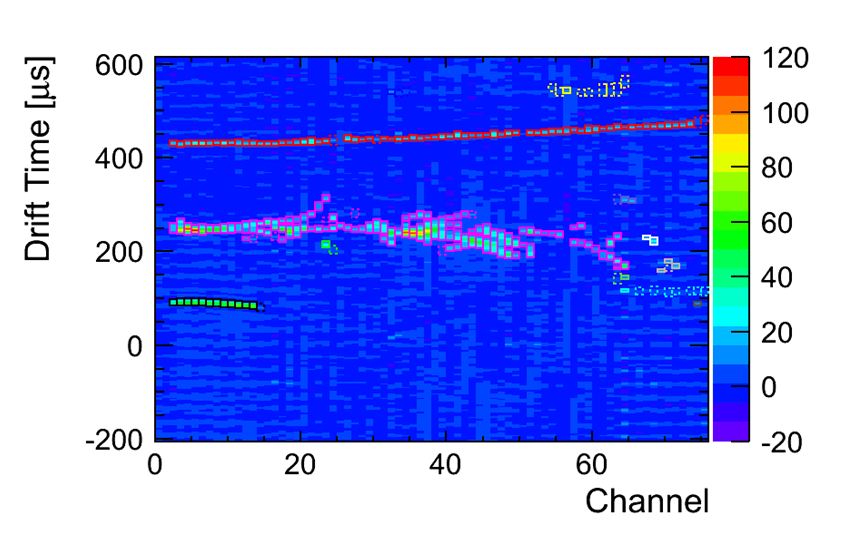
\includegraphics[width=1.0\hsize]{fig/clustering.eps}
 \end{center}
 \caption{Example of hit finding and clustering. A colored box corresponds to a hit and colors represent different clusters.}
 \label{fig:Clustering}
\end{figure}


%%%%%%%%%%%%%%%%%%%%%%%%%%%%%%%%%%%%%%%%%%%%%%%%%%
\subsection{Channel-by-Channel Calibration}
%%%%%%%%%%%%%%%%%%%%%%%%%%%%%%%%%%%%%%%%%%%%%%%%%%

Figure~\ref{fig:PionQvsCh} shows the hit charge as a function of 
the TPC channel number obtained from the 800 MeV/$c$ $\pi^+$ data. 
This figure is obtained from $\sim$300 events of well-selected Pion passing-through the TPC.
Gray-scale contours show hit charge distributions for
each channel and black points correspond to average of the hit charge distribution.  
Although we expect the energy deposition of the through-going pion to be uniform,
we observe relatively large channel dependence. 
This is mainly because of the distortion of the TPC drift field.
We use this average charge as channel-by-channel normalization scale.

\begin{figure}[htbp]
 \begin{center}
%  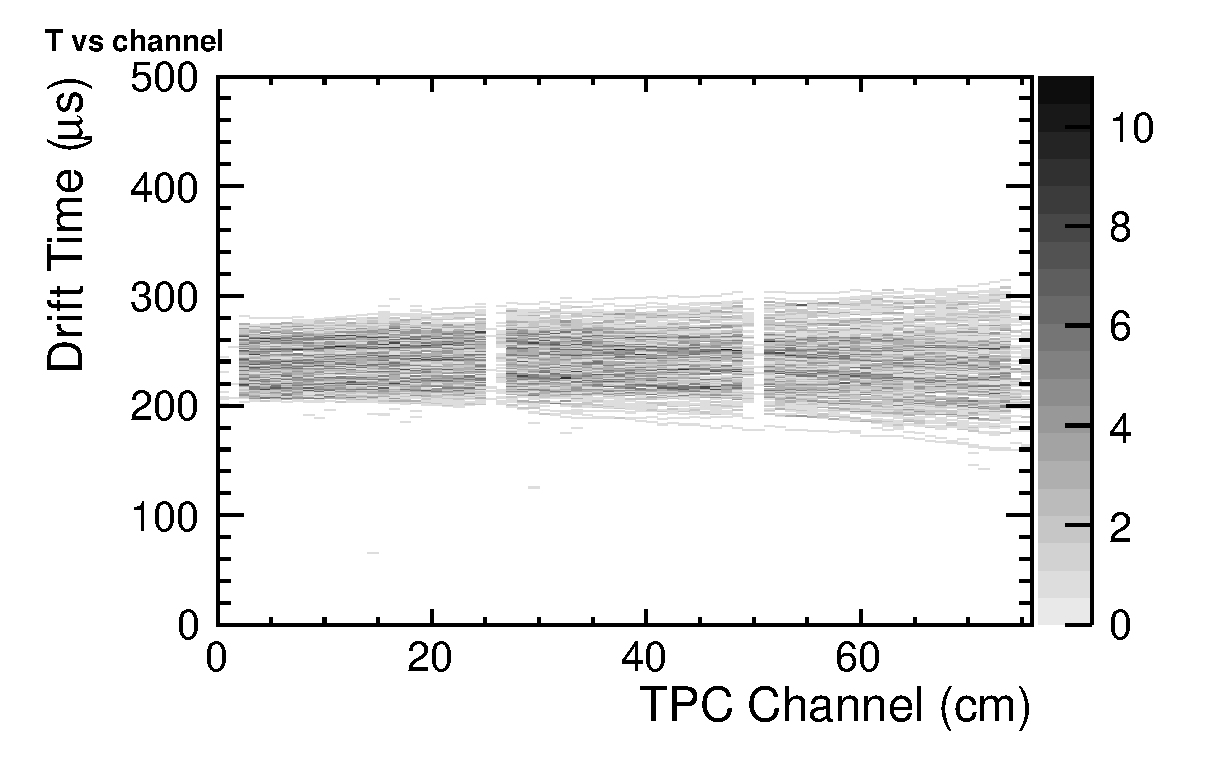
\includegraphics[width=0.8\hsize]{fig/PionTrack.eps}
  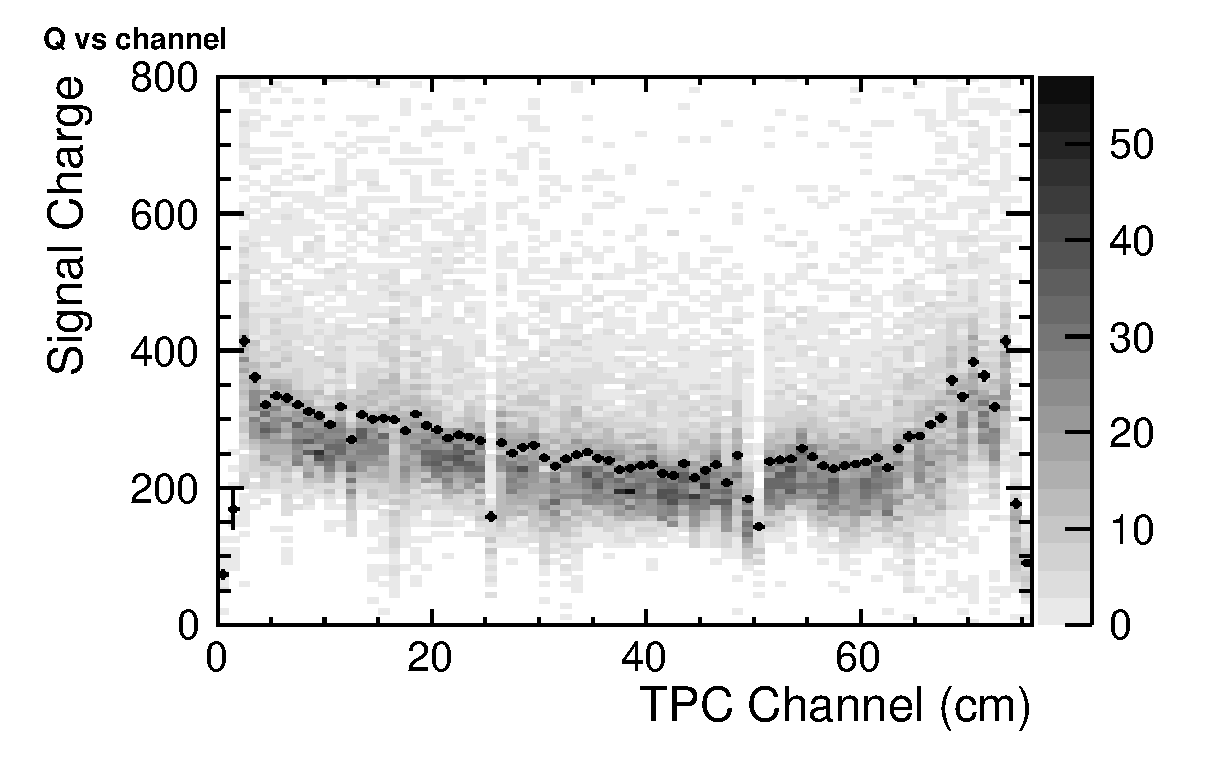
\includegraphics[width=1.0\hsize]{fig/PionQvsCh.eps}
 \end{center}
 \caption{800 MeV/c pion average hit charge}
 \label{fig:PionQvsCh}
\end{figure}

Figure~\ref{Fig:2DFieldMap} shows electric field of the TPC in V/cm which 
is calculated using a 2D FEM (Finite Element Method) package \cite{Ref:FEMTET},
where horizontal axis, vertical axis, and color strength 
correspond to the beam line direction, the drift direction, the electric field in V/cm, respectively.
Cathode, Anode, and Anode grid are located at of z=-200 mm, z=200 mm, and z=210 mm. respectively.
There are significant distortion of the electric field around 4 corners of the TPC fiducial volume,
and also around x=$\pm$120 mm where support structure of the Cathode and Anode grids exists.
We found this field distortion is the main cause of the
non-uniformity of the TPC response.

\begin{figure}[htbp]
 \begin{center}
  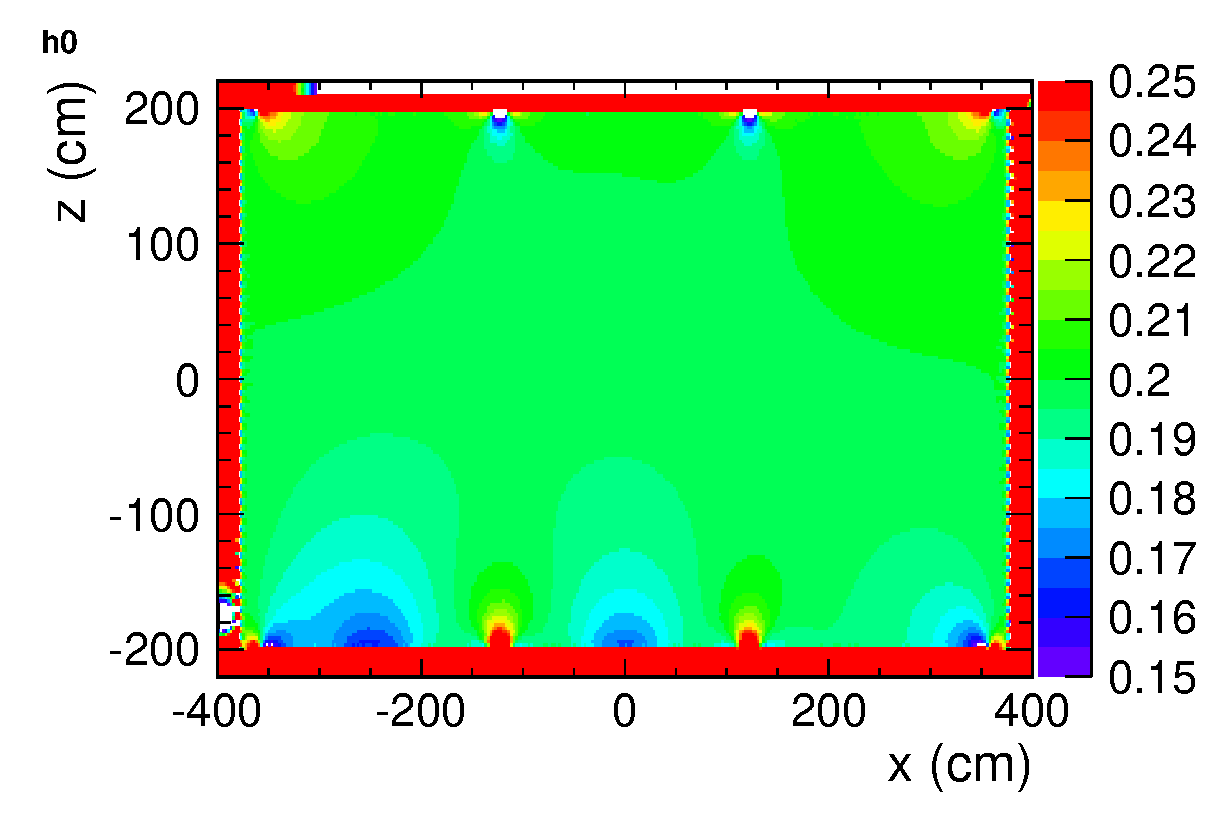
\includegraphics[width=1.0\hsize]{fig/2DFieldMap.eps}
 \end{center}
 \caption{Electric field map obtained with 2D FEM where
horizontal axis corresponds to the beam line direction,
and vertical axis corresponds to drift direction,
and color strength corresponds to electric field strength in V/cm.
}
 \label{Fig:2DFieldMap}
\end{figure}

%%%%%%%%%%%%%%%%%%%%%%%%%%%%%%%%%%%%%%%%%%%%%%%%%%
\subsection{Liquid Argon Purity}
%%%%%%%%%%%%%%%%%%%%%%%%%%%%%%%%%%%%%%%%%%%%%%%%%%

Attenuation of the drift electron depends on purity of LAr since electronegative impurities capture it \cite{purity}. 
Thus we need to apply correction to TPC signal charge according to the drift time.
We use cosmic ray events triggered by inner PMT at off-beam timing for measuring the LAr purity, and use this to correct the beam data.
Figure~\ref{fig:CosmicEvent} shows an event display of typical cosmic muon event crossing TPC channels.
The attenuation of readout charge depending on drift time is clearly seen in the right plot. 
We use multiple events to cancel Landau effect and apply channel response correction to estimate LAr purity.

\begin{figure}[htbp]
 \begin{center}
  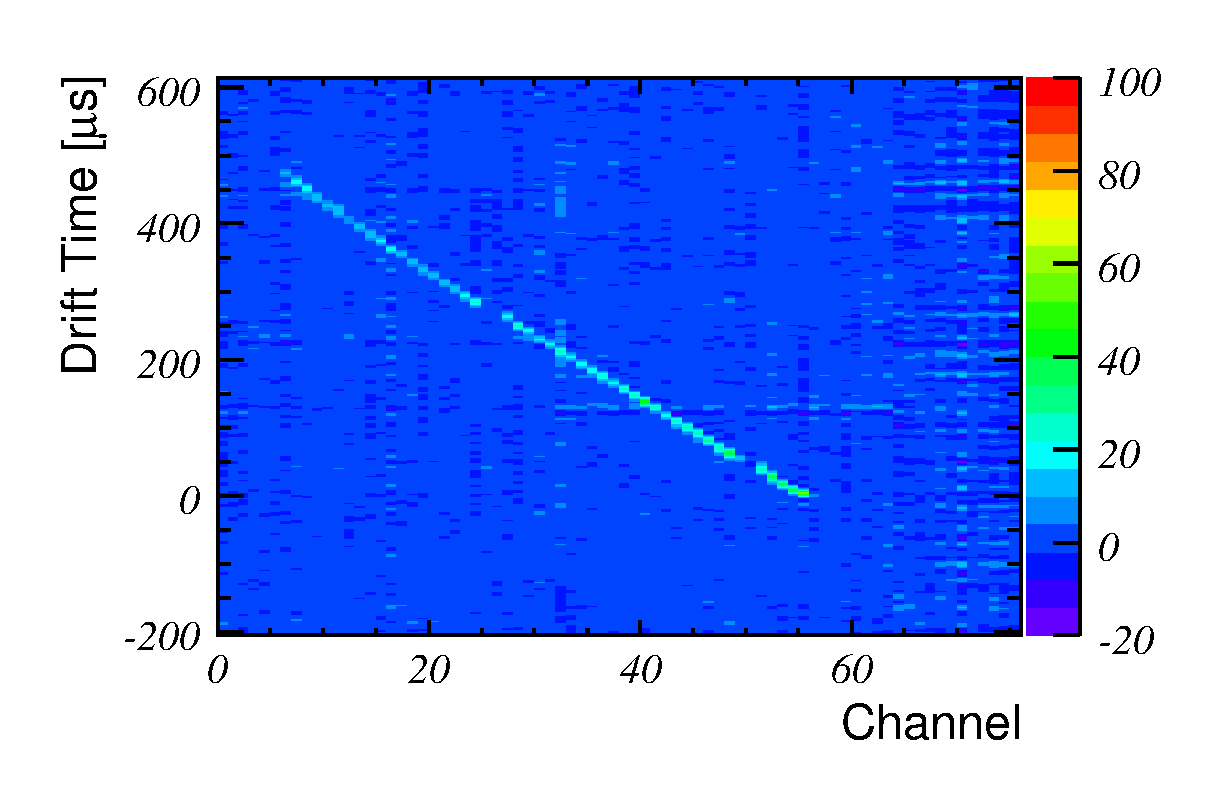
\includegraphics[width=0.49\hsize]{fig/cosmic68_ev258_display.eps}
  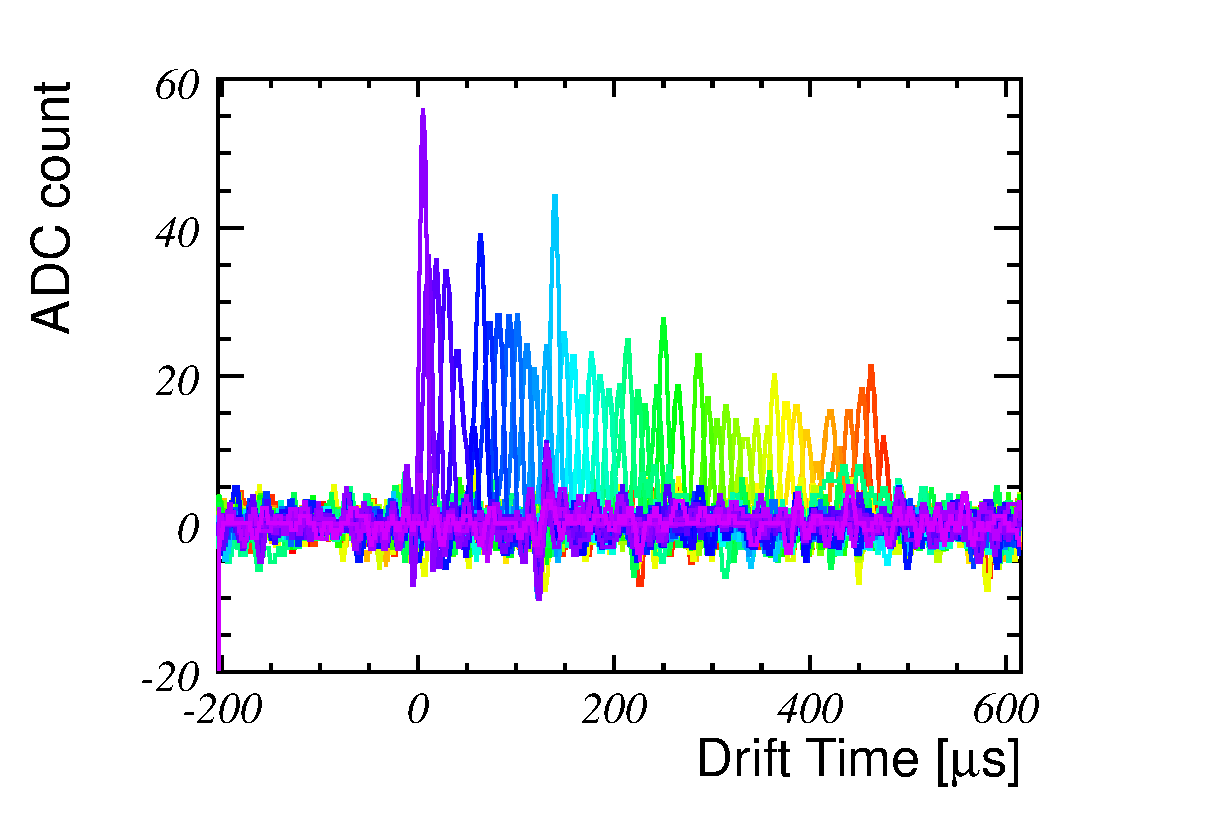
\includegraphics[width=0.49\hsize]{fig/cosmic68_ev258.eps}
 \end{center}
 \caption{Left: Typical cosmic muon event crossing TPC channels. Right: Charge deposit as a function of drift time.}
 \label{fig:CosmicEvent}
\end{figure}

We select cosmic ray event with more than 20 TPC channels which corresponds to zenith angle of more than $27^\circ$ and consistent with straight line by $\chi^2$ fit. 
%Readout charge is corrected for field distortion and projected to beam direction to correct injection angle.
We fit readout charge by Landau function in each drift time bin to estimate average charge deposit. 
%Figure~\ref{fig:tauExample} shows example of the average readout charge as a function of drift time which is fitted by exponential to obtain drift electron lifetime. 
%Realistic Monte Carlo simulation shows about 13\% (TBU) smaller lifetime estimation due to noise, field distortion, and FFT effects. 
%We correct output lifetime from these effects.
Figure~\ref{fig:CosmicPurity} shows an drift electron lifetime as a function of duration after initial LAr filling.
Drift electron lifetime was 600 $\mu$s at 60 hours, and 400 $\mu$s after 150 hours.
%Initial purity looks good, but the purity was slowly degrading while data taking period.
The degradation is possibly due to impurity from micro leak or out-gassing penetrating faster than purification by gas recirculation.
But we kept enough drift electron lifetime during data taking period.
The effects from noise, field distortion, and FFT give about 10\% (to be confirmed) of systematic uncertainty in LAr purity estimation.
%Since charge in simulation is calibrated using through-going $\pi$ data as described later and duration of analyzed beam data is short (about 30 hours), this uncertainty gives negligible effects (to be updated, show percentage) in beam data analysis. 

%\begin{figure}[htbp]
% \begin{center}
%  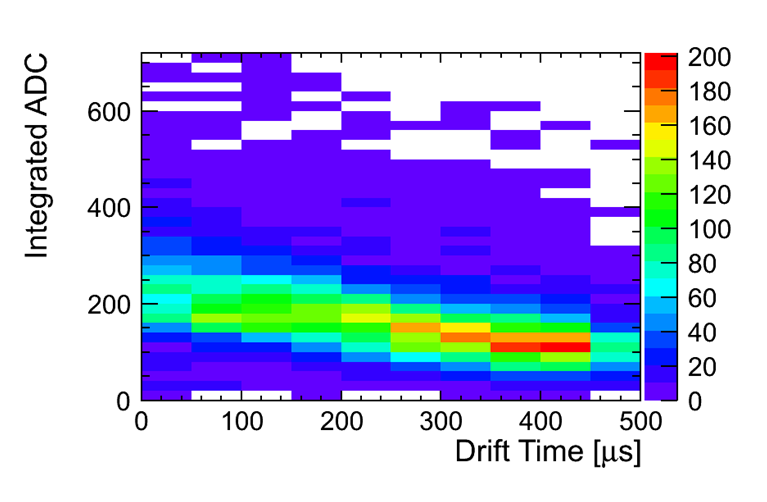
\includegraphics[width=0.45\hsize]{fig/chargeDep.eps}
%  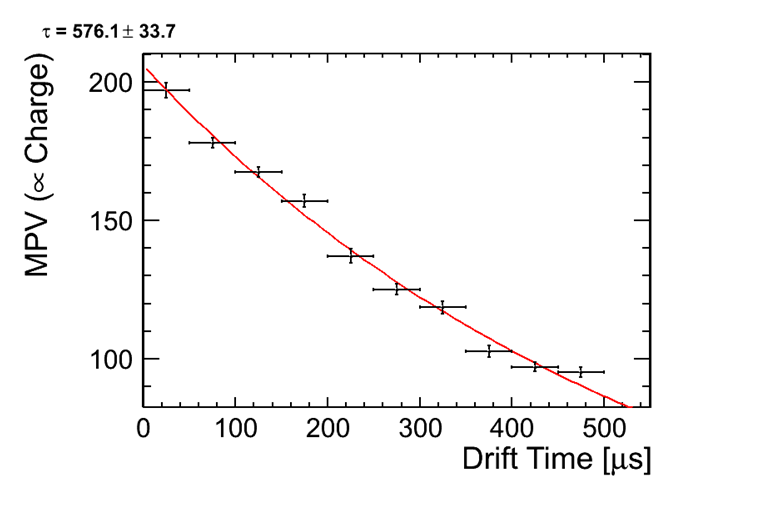
\includegraphics[width=0.45\hsize]{fig/tauExample.eps}
% \end{center}
% \caption{Left: Readout charge as a function of drift time. Readout charge in each drift time bin is fitted by landau function. Right: Average charge readout as a function of drift time which is fitted by exponential to estimate drift electron lifetime.}
% \label{fig:tauExample}
%\end{figure}

\begin{figure}[htbp]
 \begin{center}
  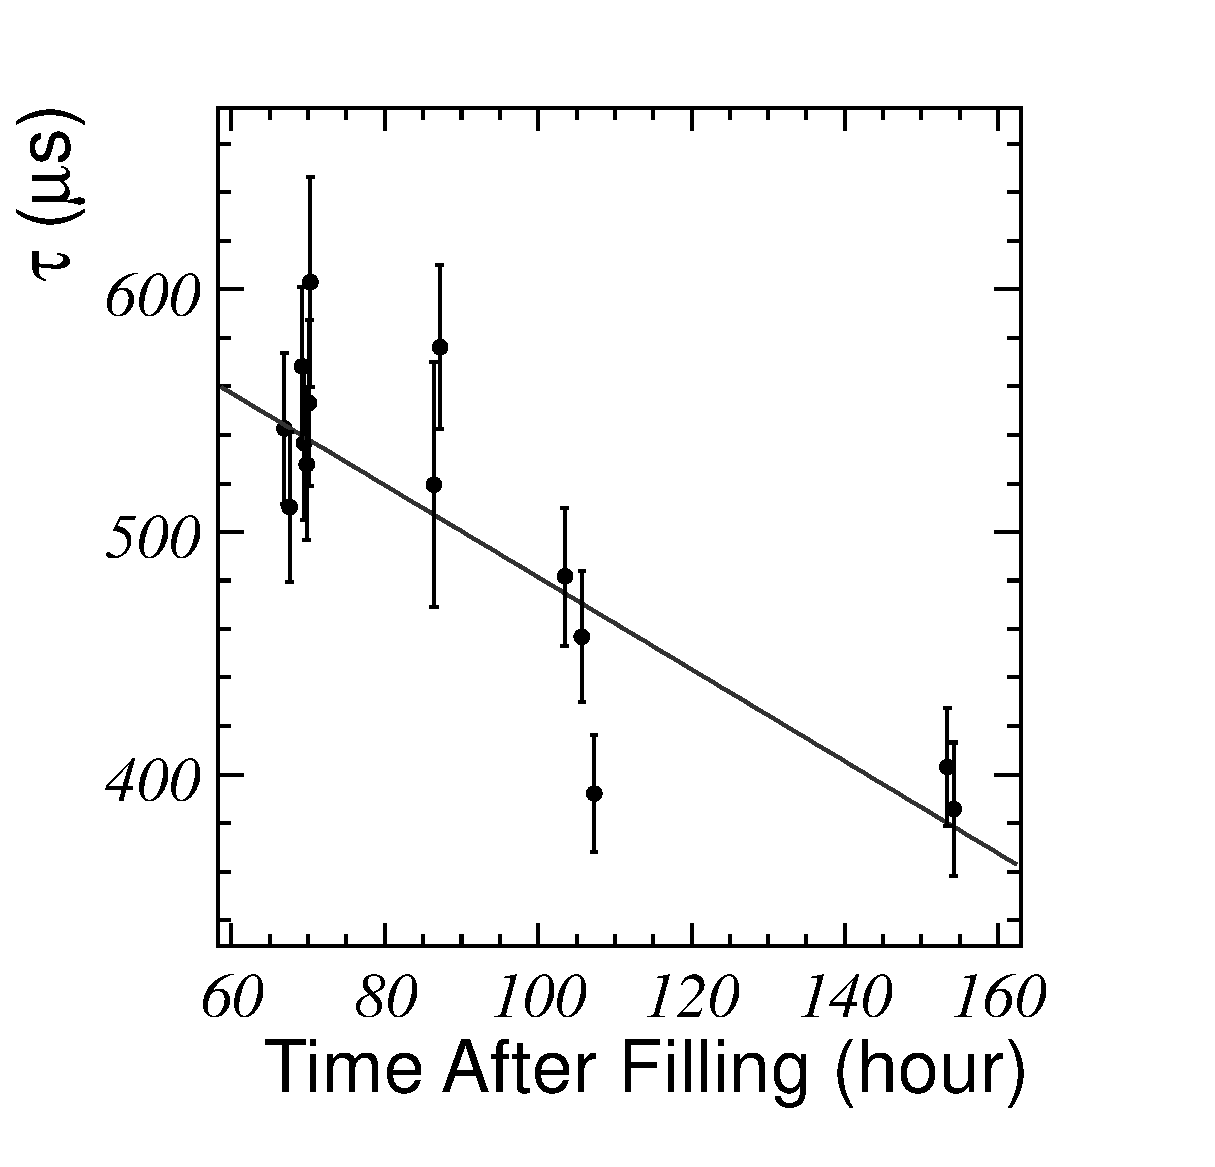
\includegraphics[width=1.0\hsize]{fig/tauHistory.eps}
 \end{center}
 \caption{Drift electron lifetime as a function of duration after initial LAr filling. The lifetime is used to correct the beam data.}
 \label{fig:CosmicPurity}
\end{figure}

\subsection{Cross Talk}

TBD

%Figure\ref{fig:cross_talk1} shows the signal wave form of stopped channel and the front channel of typical proton event.
%The signal wave form of stopped channel is differential form of the that of the front channel.
%Such signals are appeared at channel number 1 which cannot enter drifted ionization electron in electric power lines.
%One possibility which cause such a phenomenon is following process.
%The distance between anode channels is very short,
%so the influence of mutual capacitance become large
%and this capacitive coupling induce cross talk noise.
%This effect notably appears the channel where the difference of the charge between adjacent channels is large,
%such as the channel around stopped point of proton.
%Then, we implement this phenomenon in Monte Carlo Simulation
%by adding bipolar shape of the signal Gavin shape at adjacent channels.
%The area of the mountain of bipolar shape is 10.5\% of the area of signal Gaussian at each adjacent channel.
%The value of 10.5\% is determined by comparing the hit charge distribution at stopped channel between data and MC simulation.
%Figure\ref{fig:cross_talk2} shows hit charge distribution of stopped channel.
%Black is data and blue is MC simulation with cross talk red is MC simulation without cross talk.
%As fig\ref{fig:cross_talk2} shown, data and MC simulation with cross talk is good agreement,
%so the value of 10.5\% is reasonable.

\begin{figure}[htbp]
  \begin{center}
    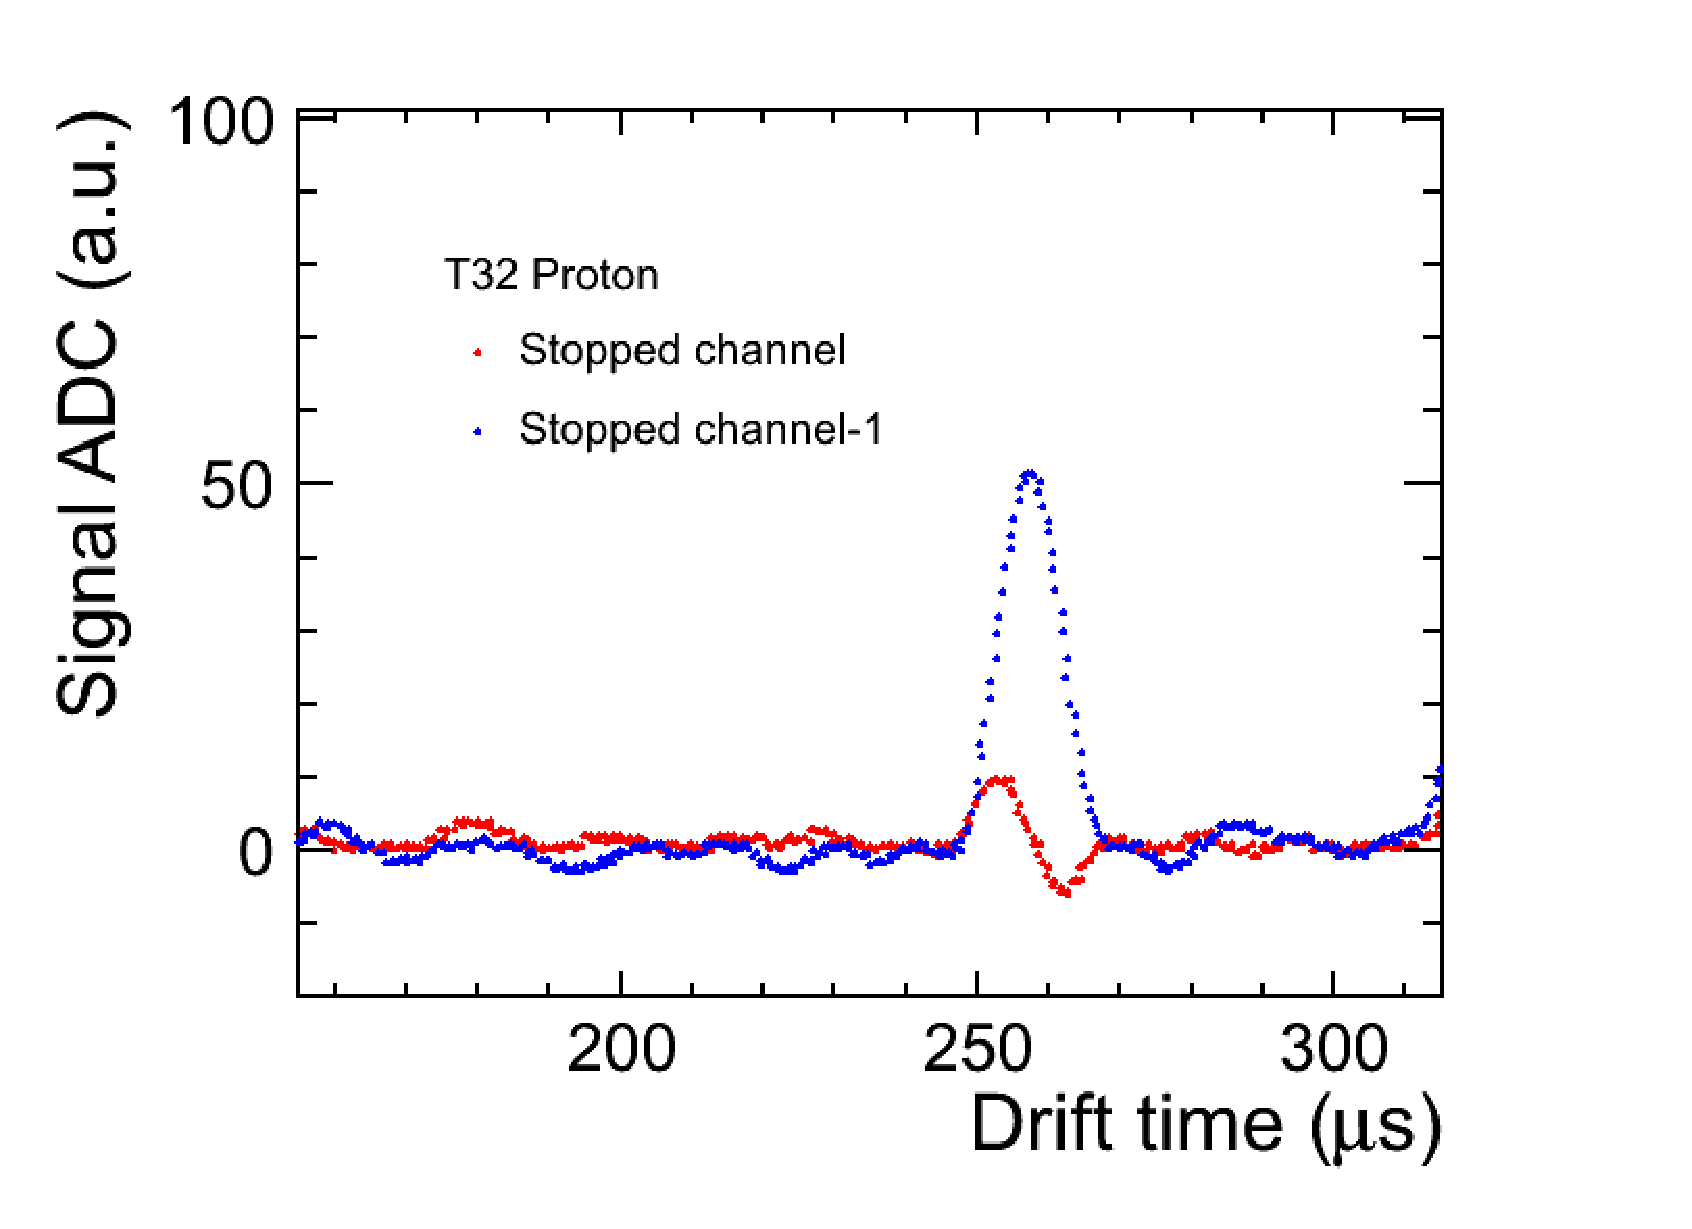
\includegraphics[width=1.0\hsize,clip]{fig/cross_talk_1.eps}
%    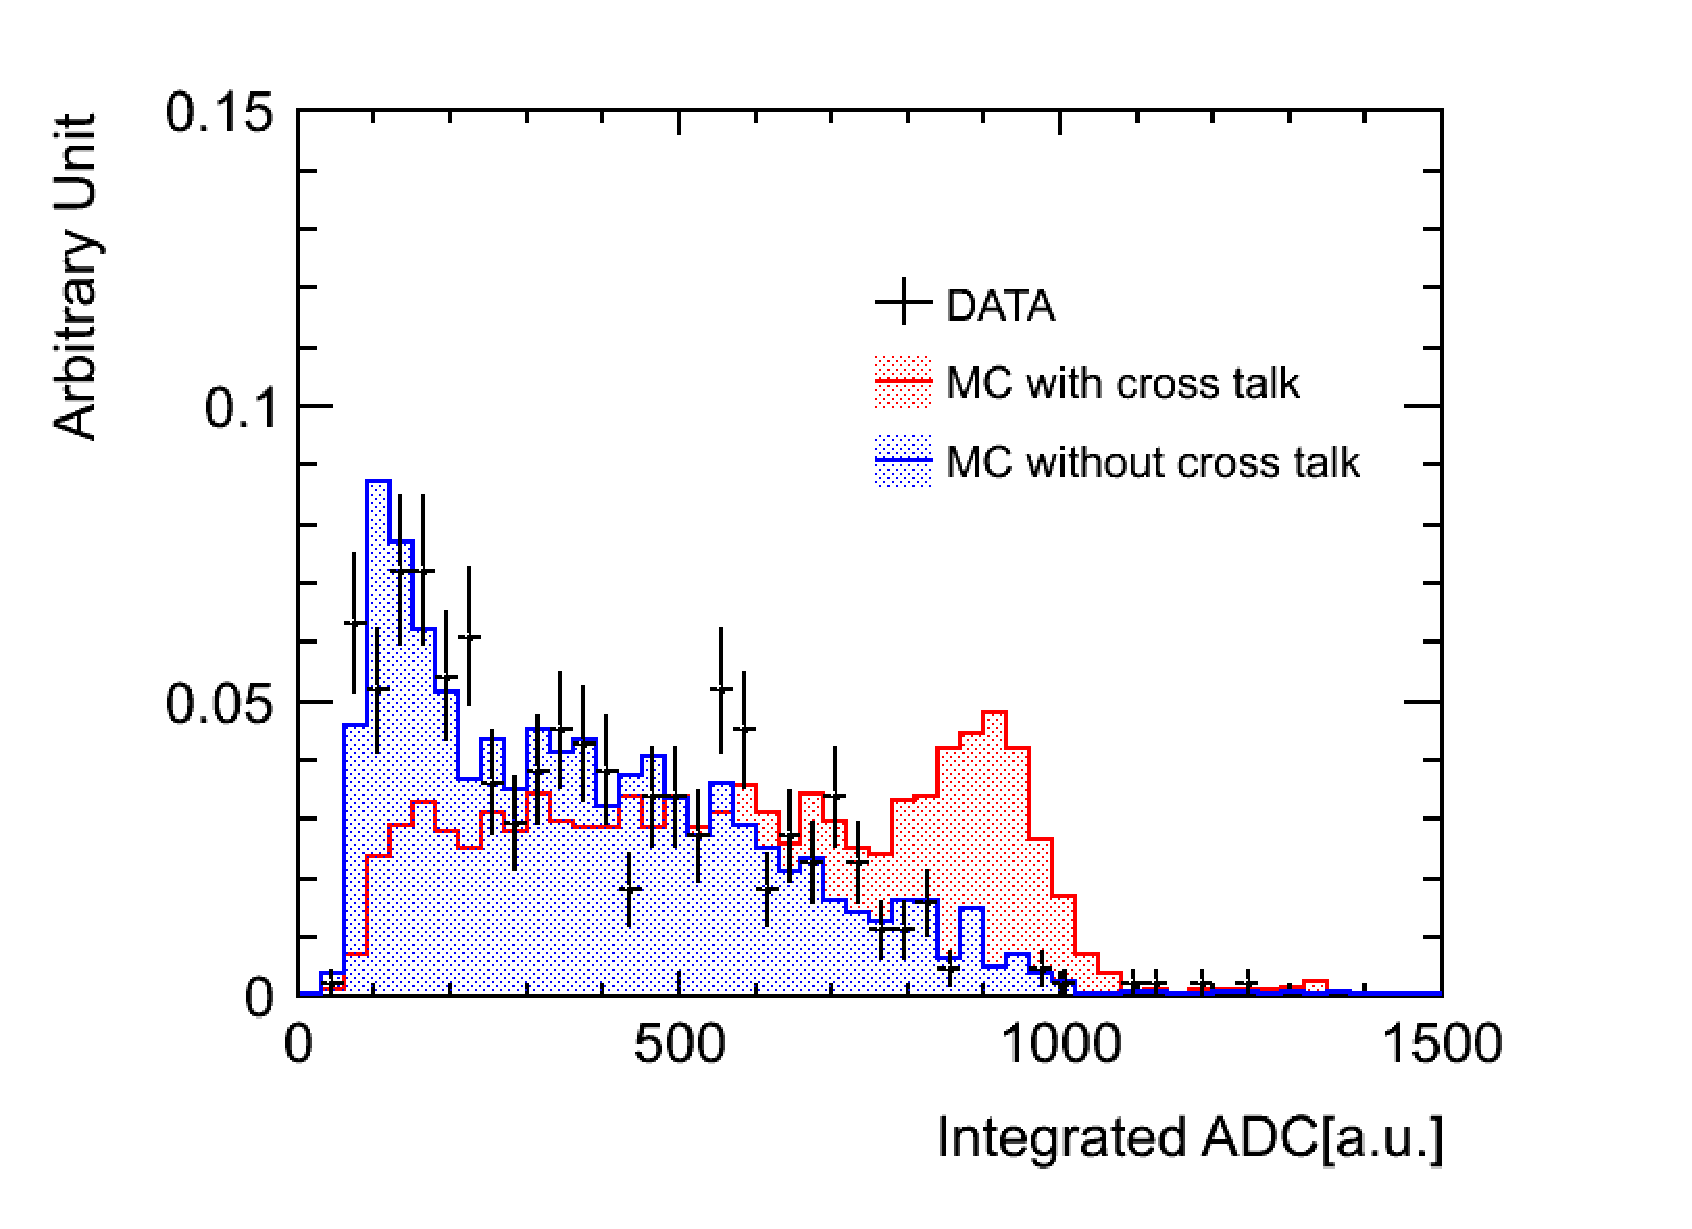
\includegraphics[width=0.45\hsize,clip]{fig/cross_talk_2.eps}
  \end{center}
  \caption{Left plot shows signal wave form of stopped channel and the front channel, 
    and right plot shows hit charge distribution of stopped channel}
  \label{fig:cross_talk1}
  \label{fig:cross_talk2}
\end{figure}

%%%%%%%%%%%%%%%%%%%%%%%%%%%%%%%%%%%%%%%%%%%%%%%%%%
%\section{Simulation}
%%%%%%%%%%%%%%%%%%%%%%%%%%%%%%%%%%%%%%%%%%%%%%%%%%
%%%%%%%%%%%%%%%%%%%%%%%%%%%%%%%%%%%%%%%%%%%%%%%%%%
\section{Simulation Sample}
%%%%%%%%%%%%%%%%%%%%%%%%%%%%%%%%%%%%%%%%%%%%%%%%%%
Development of the realistic simulation is one of the main task of this experiment.
We try to put all the effects (Field distortion, LAr purity, cross talk, etc) into this simulation,
and see if the properties of LArTPC in data can be reproduced using the simulated sample.

\label{Sec:Simulation}
\subsection{Signal Simulation}
We use GEANT3 for simulating energy deposition of initial beam particles and
secondary particles to the TPC detector and beam line counters. 
Maximum step of GEANT is set to 0.5 mm which is enough smaller than the TPC readout pitch of 1 cm.
We set energy cut-off for soft electron/photon emission to 10 keV which is minimum possible energy can be set in GEANT3.
Recombination of electron and Argon ion depends on the electric field $E$ and $dE/dx$, and explained by the following equation (Birks law)
\begin{equation}
  Q = A\frac{Q_{0}}{1+(k/E)\times(dE/dx)\times(1/\rho)}
\label{eq:birkslaw}
\end{equation}
where $Q_{0}$ is initial ionization charge, $\rho$ is density of liquid Argon (=1.4 g/cm$^3$).
For $A$ and $k$, we use the measurement by ICARUS collaboration \cite{658352}.
Electric field is given by Fig.\ref{Fig:2DFieldMap}.

After the recombination, drift of the ionization electrons to anode is simulated
using a simple step simulation with step size of 0.1 mm.
Drift velocity of the ionization electron depends on the liquid Argon temperature,
and the electric field. We use a measurement by ICARUS collaboration \cite{649233}, and
electric field in Fig.\ref{Fig:2DFieldMap}. 
Typical drift velocity with 200 V/cm of the drift field and temperature of 92K is 0.8 m/ms.
Diffusion of the drift electron is considered and we assume coefficient for the transverse diffusion 
and and lateral diffusion are 9.0 mm$^2$/m and 2.3 mm$^2$/m, respectively (need reference).

\begin{itemize}
\item Simulate Signal waveform: Gaussian
\end{itemize}
simulation of recombination, drift, waveform is done for every GEANT step, and
the resulting waveform is summed up for all the particles in the event.
After ending of the event process, noise waveform which describes in the next section is added to the signal waveform,
and then the signal charge is digitized.

%Figure~\ref{Fig:DriftSimulation} shows simulated track of the drift electrons with three different positions.
%left plot with x= 0 mm corresponds to the center of the TPC detector, 
%middle plot with x= 130 mm corresponds to the location of anode grid frame,
%and right plot with x= 350 mm corresponds to the edge of the TPC fiducial.
%Because of the field distortion we find significant displacement of the drift electron in
%x direction for x=130 and x=350. It is a main source of the non-uniformity observed in 
%the through-going pion response (Fig.~\ref{fig:PionQvsCh}).

%\begin{figure}[htbp]
% \begin{center}
%  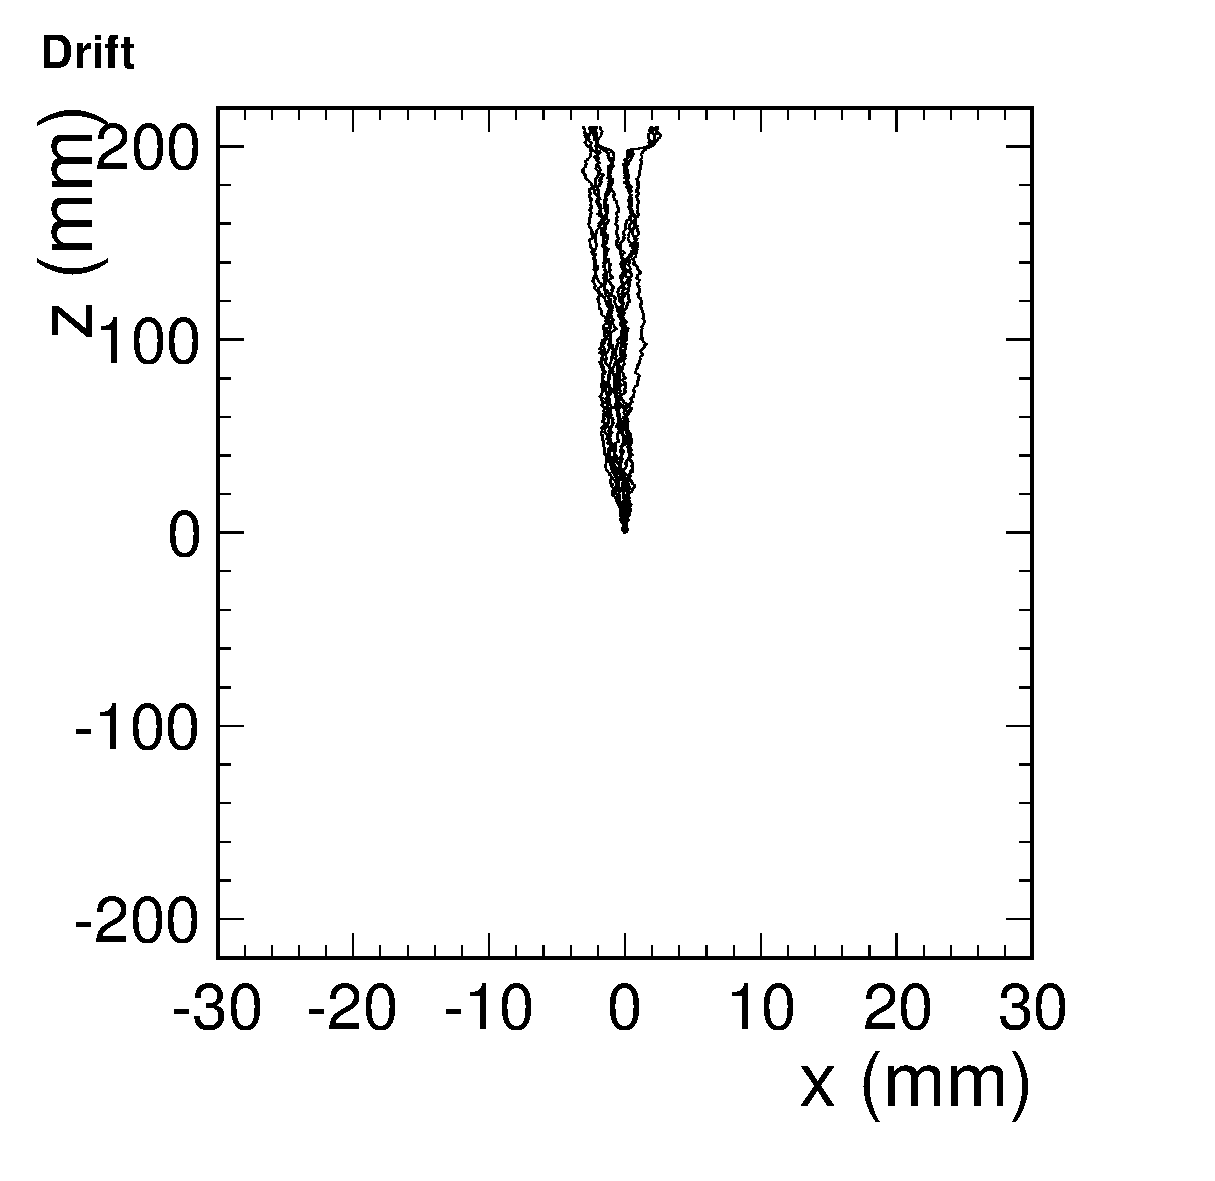
\includegraphics[width=0.3\hsize]{fig/Drift_0.eps}
%  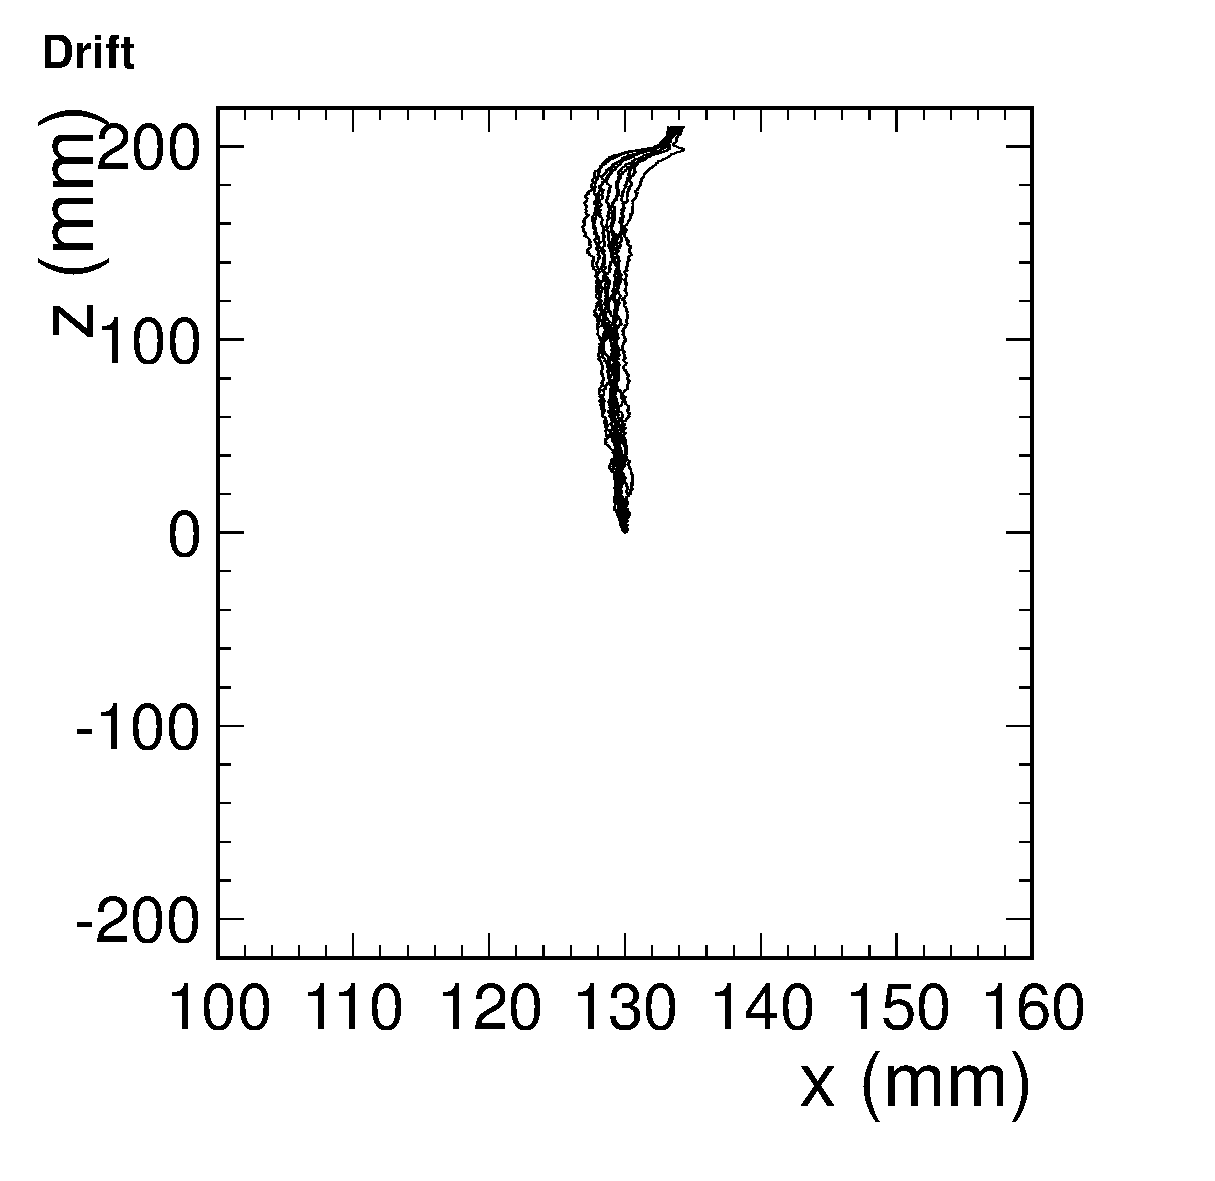
\includegraphics[width=0.3\hsize]{fig/Drift_130.eps}
%  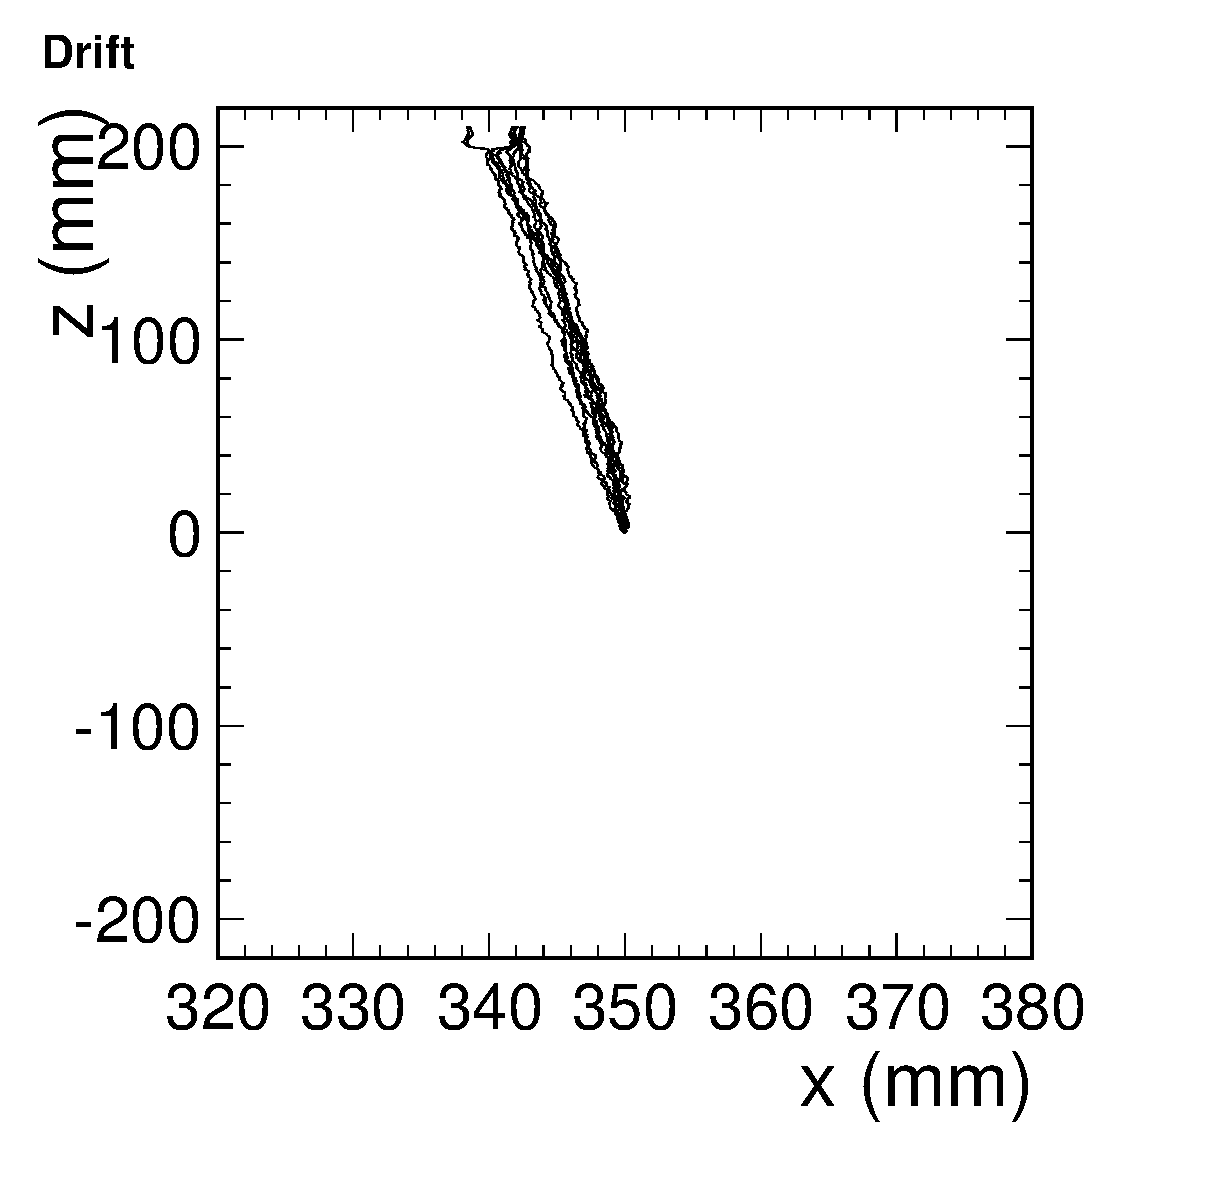
\includegraphics[width=0.3\hsize]{fig/Drift_350.eps}
% \end{center}
% \caption{Simulation of the electron drift with three different initial positions. Left, middle, and right plots corresponds to x=0, x=130 mm, and x=350 mm, respectively.}
% \label{Fig:DriftSimulation}
%\end{figure}

%\begin{itemize}
%\item Plot: drift simulation  (Tanaka)
%\end{itemize}
%\subsection{Preamp Response and Digitization}
%\begin{itemize}
%\item Preamp gain vs channel number  (Naito)
%\end{itemize}

%\subsection{FFT Noise}
%\subsection{FFT Noise}
There are two kinds of noise in the data we obtained, random noise and coherent noise.
Random noise is the noise which exists in each anode channel.
Coherent noise is in each board.
The pseudo noise we implemented in Monte Carlo simulation is composed of random and coherent noise by this reason.

Random noise is generated from FFT(Fast Fourier Transform) distribution of real data. Figure \ref{example10ch} shows an example of FFT distribution.

Coherent noise is generated board by board as the noise scale in the real data we obtained.
The noise scale is defined as a root mean square of pedestal, minimum noise scale is about 3 and maximum noise scale is about 10 in the data.

The ratio of random and coherent noise is 1:1 as equation \ref{PseudoNoise}.
Figure \ref{DATAnoise} shows real data noise and Fig.\ref{MCnoise} shows pseudo noise we implemented in Monte Carlo simulation.
\begin{equation}
  Pseudo\,Noise = \frac{Random\,Noise + Coherent\,Noise}{2}
  \label{PseudoNoise}
\end{equation}

\begin{figure}[!htb]
  \centering
  \centering
  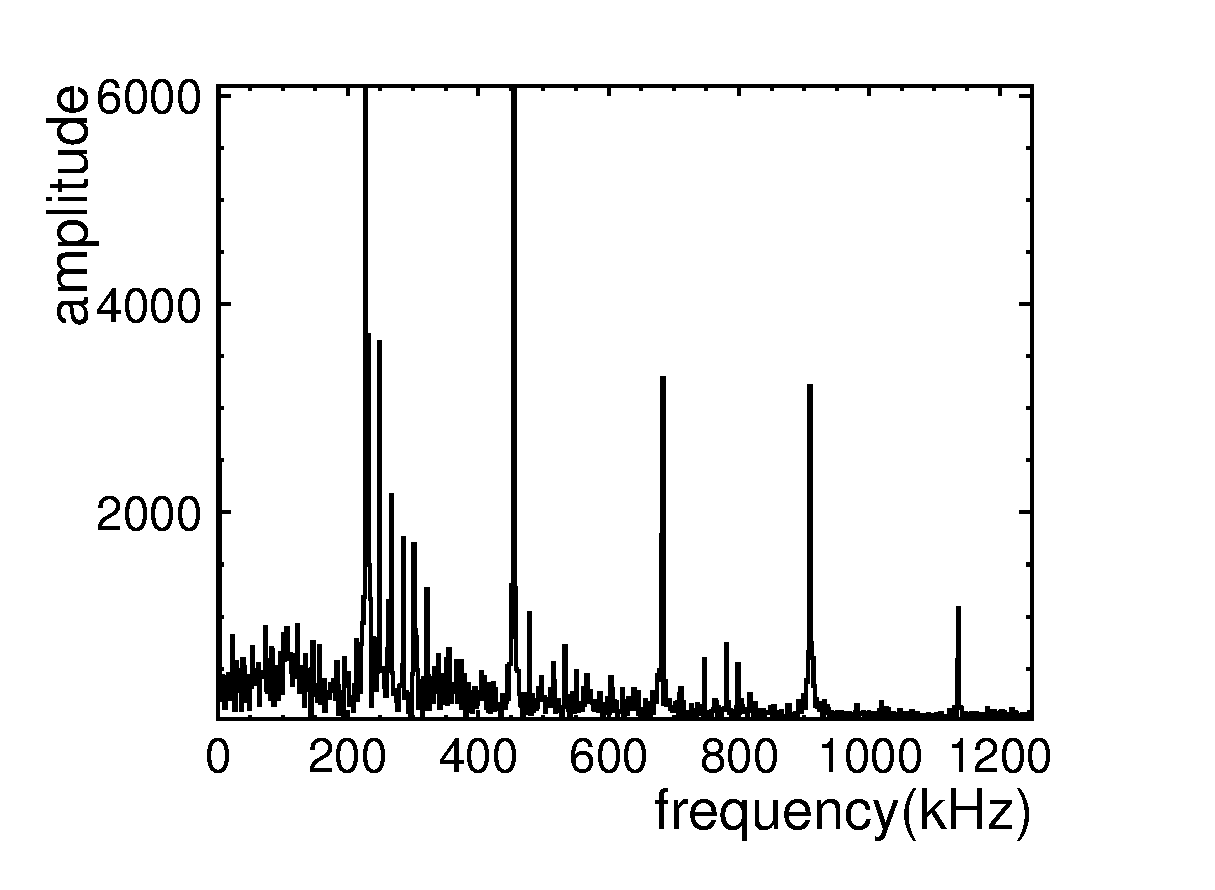
\includegraphics[width=10cm,clip]{./fig/FFTdist.eps}
  \caption{An example distribution of frequency}
  \label{example10ch}
\end{figure}
%\begin{figure}[!htb]
%  \centering
%  \centering
%  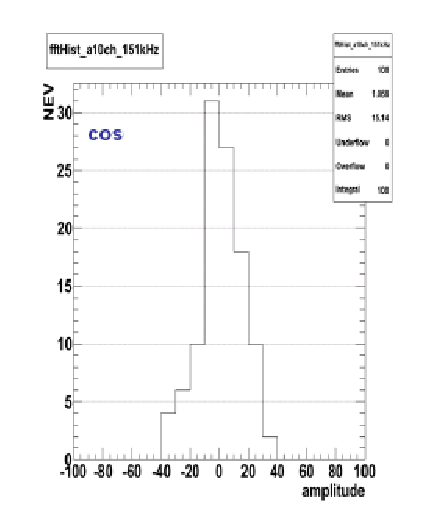
\includegraphics[width=11cm,clip]{./fig/cos.eps}
%  \caption{An example of distribution of amplitude}
%  \label{ampDist}
%\end{figure}
%\begin{figure}[!htb]
%  \centering
%  \centering
%  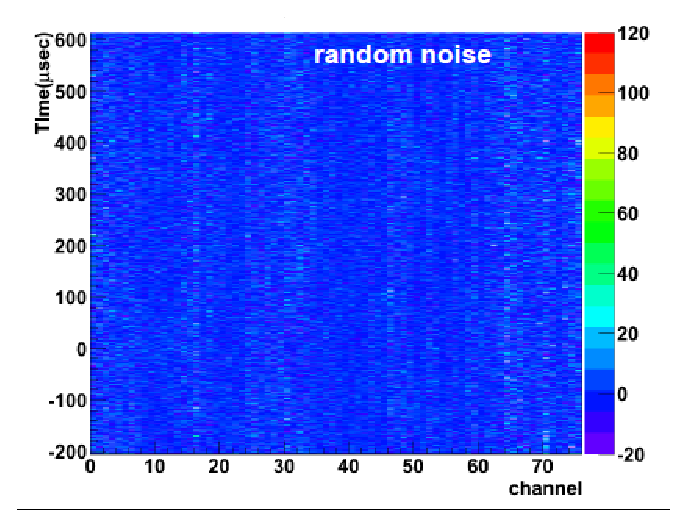
\includegraphics[width=11cm,clip]{./fig/randomnoise.eps}
%  \caption{Random noise}
%  \label{randomNoise}
%\end{figure}
\begin{figure}[!htb]
\begin{minipage}{0.5\hsize}
  \centering
  \includegraphics[width=7cm,clip]{./fig/DATAnoise.eps}
  \caption{Data noise}
  \label{DATAnoise}
\end{minipage}
\begin{minipage}{0.5\hsize}
  \centering
  \includegraphics[width=7cm,clip]{./fig/MCnoise.eps}
  \caption{Pseudo noise(Noise simulation)}
  \label{MCnoise}
\end{minipage}
\end{figure}
%\begin{figure}[!htb]
%  \centering
%  \centering
%  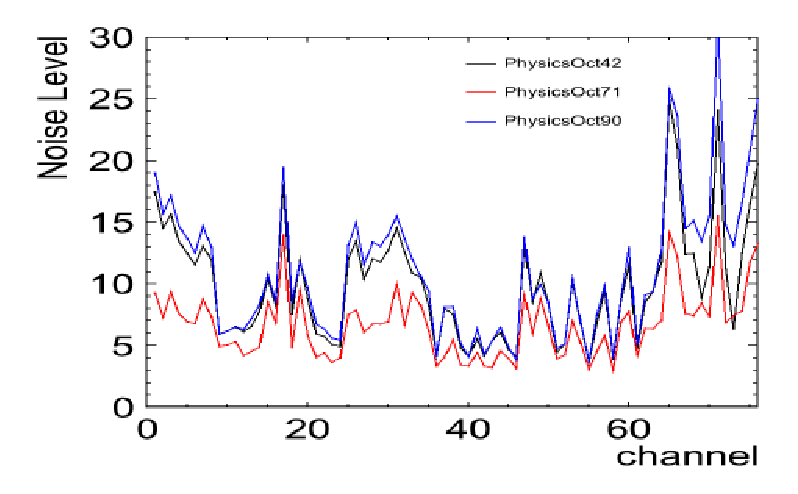
\includegraphics[width=11cm,clip]{./fig/scaling.eps}
%  \caption{Noise level}
%  \label{scaling}
%\end{figure}
\subsection{Noise Simulation}

\begin{itemize}
\item We generate noise from FFT amplitude distribution such as in Fig.\ref{Fig:FFT}
\item By using empty event, prepare template distribution of amplitude for each channel and each frequency bin
\item Obtain waveform by generating random number from the template
\item Coherent noise is added board by board
\end{itemize}

%There are two kinds of noise in the data we obtained, random noise and coherent noise.
%Random noise is the noise which exists in each anode channel.
%Coherent noise is in each board.
%The pseudo noise we implemented in Monte Carlo simulation is composed of random and coherent noise by this reason.

%Random noise is generated from FFT distribution of real data (See Fig.\ref{fig:FFT}).

%Coherent noise is generated board by board as the noise scale in the real data we obtained.
%The noise scale is defined as a root mean square of pedestal, minimum noise scale is about 3 and maximum noise scale is about 10 in the data.

%The ratio of random and coherent noise is 1:1 as equation \ref{PseudoNoise}.
%Figure \ref{DATAnoise} shows real data noise and Fig.\ref{MCnoise} shows pseudo noise we implemented in Monte Carlo simulation.
%\begin{equation}
%  Pseudo\,Noise = \frac{Random\,Noise + Coherent\,Noise}{2}
%  \label{PseudoNoise}
%\end{equation}

%\begin{figure}[!htb]
%  \centering
%  \centering
%  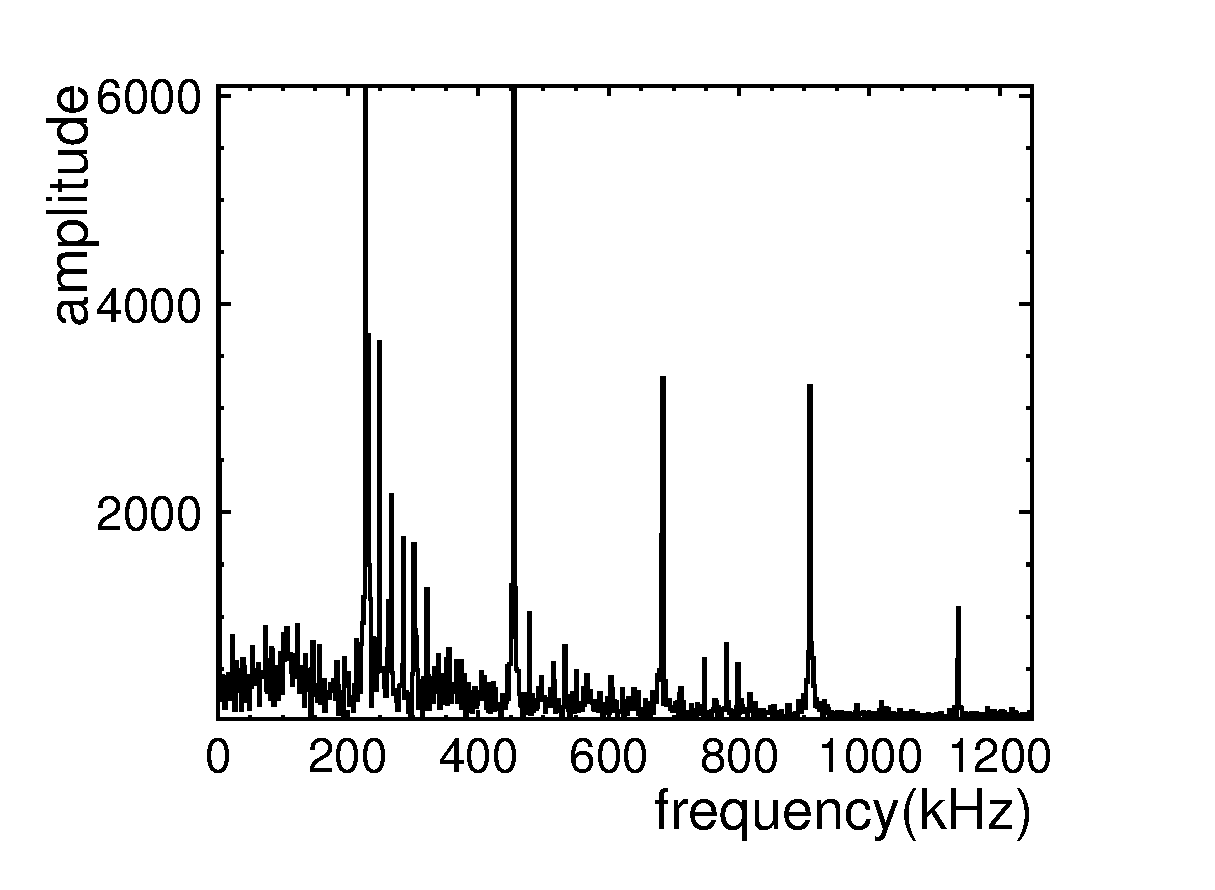
\includegraphics[width=10cm,clip]{./fig/FFTdist.eps}
%  \caption{An example distribution of frequency}
%  \label{example10ch}
%\end{figure}
%\begin{figure}[!htb]
%  \centering
%  \centering
%  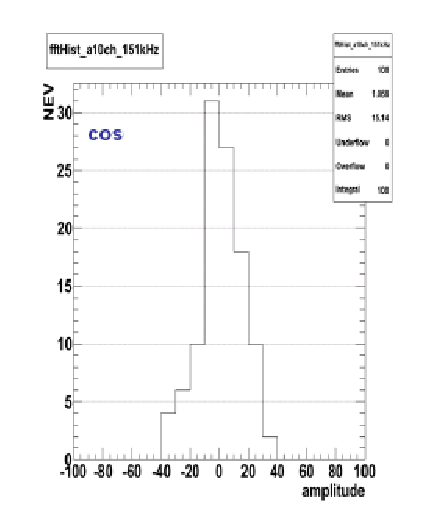
\includegraphics[width=11cm,clip]{./fig/cos.eps}
%  \caption{An example of distribution of amplitude}
%  \label{ampDist}
%\end{figure}
%\begin{figure}[!htb]
%  \centering
%  \centering
%  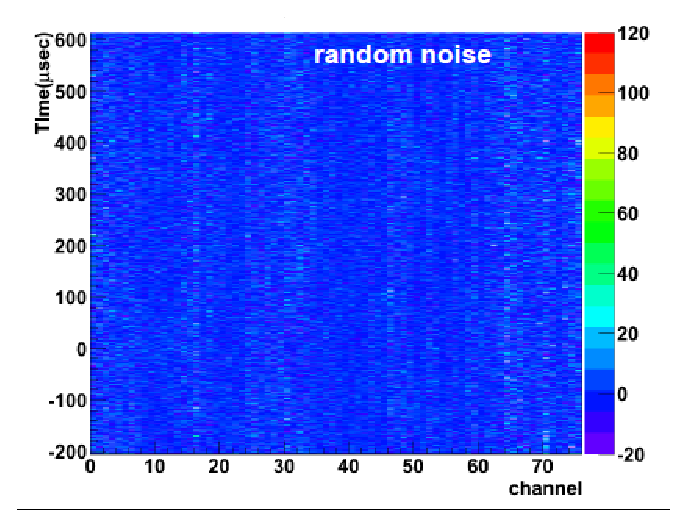
\includegraphics[width=11cm,clip]{./fig/randomnoise.eps}
%  \caption{Random noise}
%  \label{randomNoise}
%\end{figure}
%\begin{figure}[!htb]
%  \begin{center}
%    \includegraphics[width=0.45\hsize,clip]{./fig/DATAnoise.eps}
%    \includegraphics[width=0.45\hsize,clip]{./fig/MCnoise.eps}
%  \end{center}
%  \caption{Noise}
%  \label{DATAnoise}
%  \label{MCnoise}
%\end{figure}
%\begin{figure}[!htb]
%  \centering
%  \centering
%  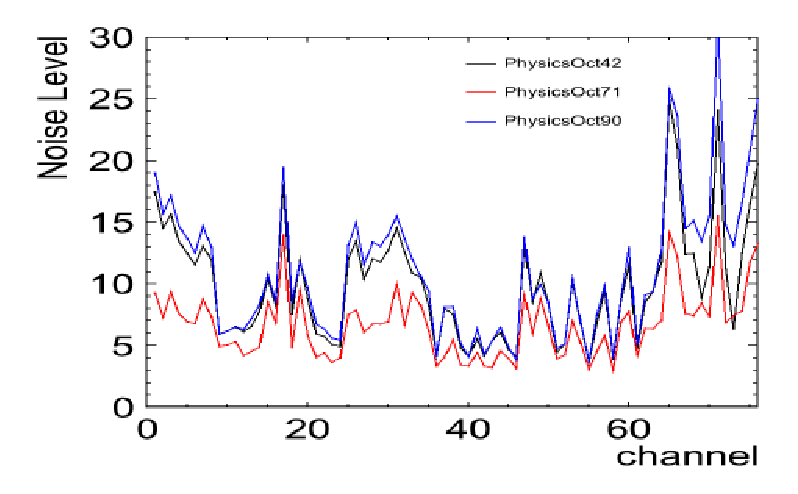
\includegraphics[width=11cm,clip]{./fig/scaling.eps}
%  \caption{Noise level}
%  \label{scaling}
%\end{figure}

Figure~\ref{Fig:SimulatedKaon} shows simulated event of 630 MeV/$c$ $K^+\to\mu\nu$.

\begin{figure}[htbp]
 \begin{center}
  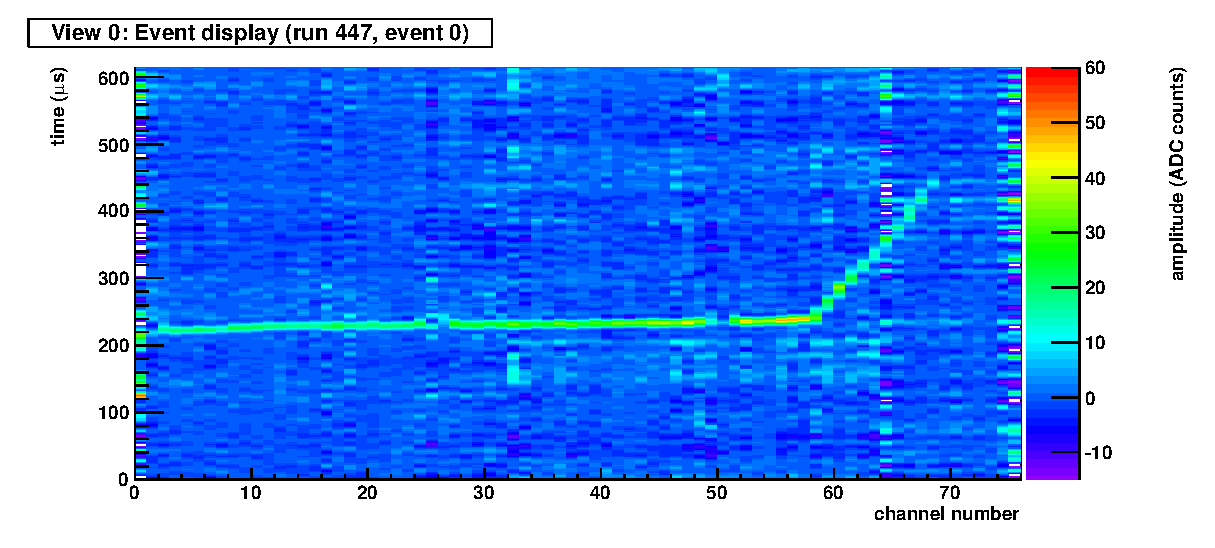
\includegraphics[width=0.8\hsize]{fig/Simulation.eps}
 \end{center}
 \caption{Event display of simulated events for 630 MeV/$c$ $K^+$.}
 \label{Fig:SimulatedKaon}
\end{figure}


%\subsection{Beam energy}
We estimated a beam momentum using simple MC simulation.
Figure \ref{K11Br_Beam_line} shows MC simulation's geometry.
We generate 800MeV/$c$ pencil beam and shoot the beam downstream.
Figure \ref{k_pi_momentum} shows Kaon and Pion momentum distribution
using this MC simulation at BDC.
Kaon beam momentum is estimated by the momentum distribution of MC simulation.
%Actually, kaon momentum distribution peak is adjusted so that kaon decay point of MC simulation is consistent with data.
%Section \ref{kaon_energy_section} explains this point.
%And proton momentum is estimated in other way, using TREK detector TOF information.
%Section \ref{proton_energy_section} shows proton momentum distribution.

\begin{figure}[!htb]
  \centering
  \centering
  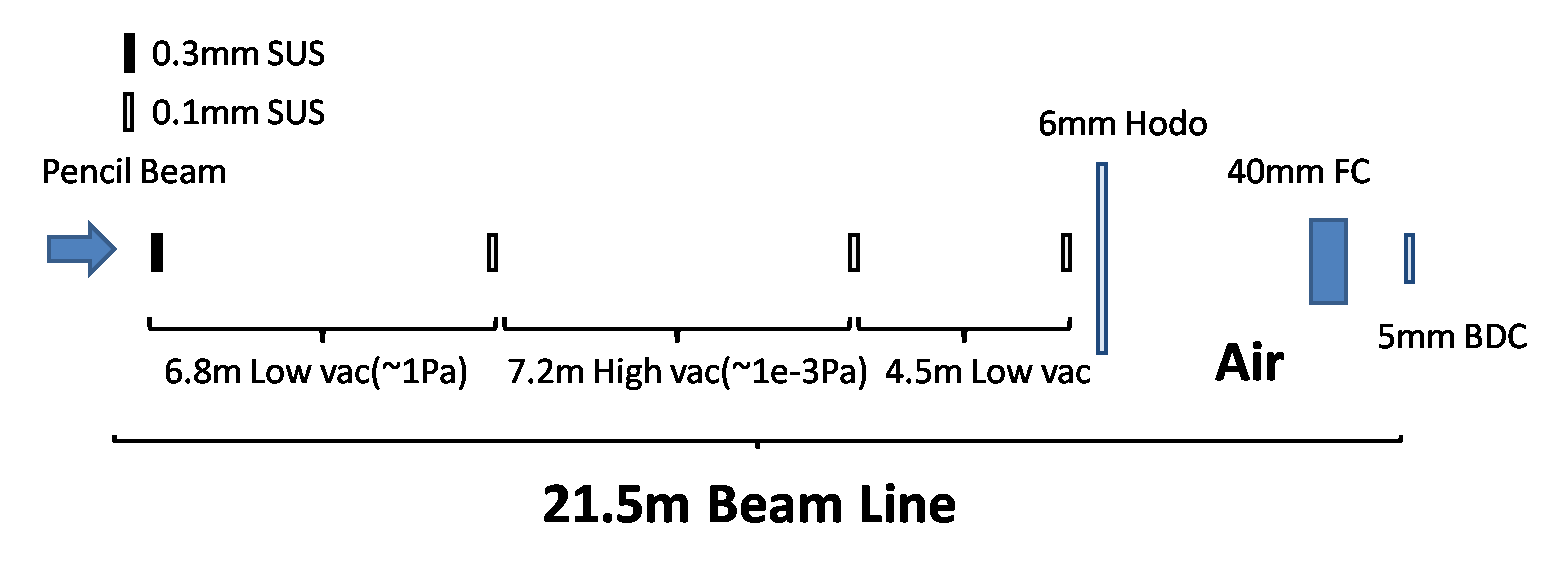
\includegraphics[width=10cm,clip]{./fig/K11Br_beamline_sim.eps}
  \caption{K1.1 Br beam line}
  \label{K11Br_Beam_line}
\end{figure}


\begin{figure}[!htb]
  \centering
  \centering
  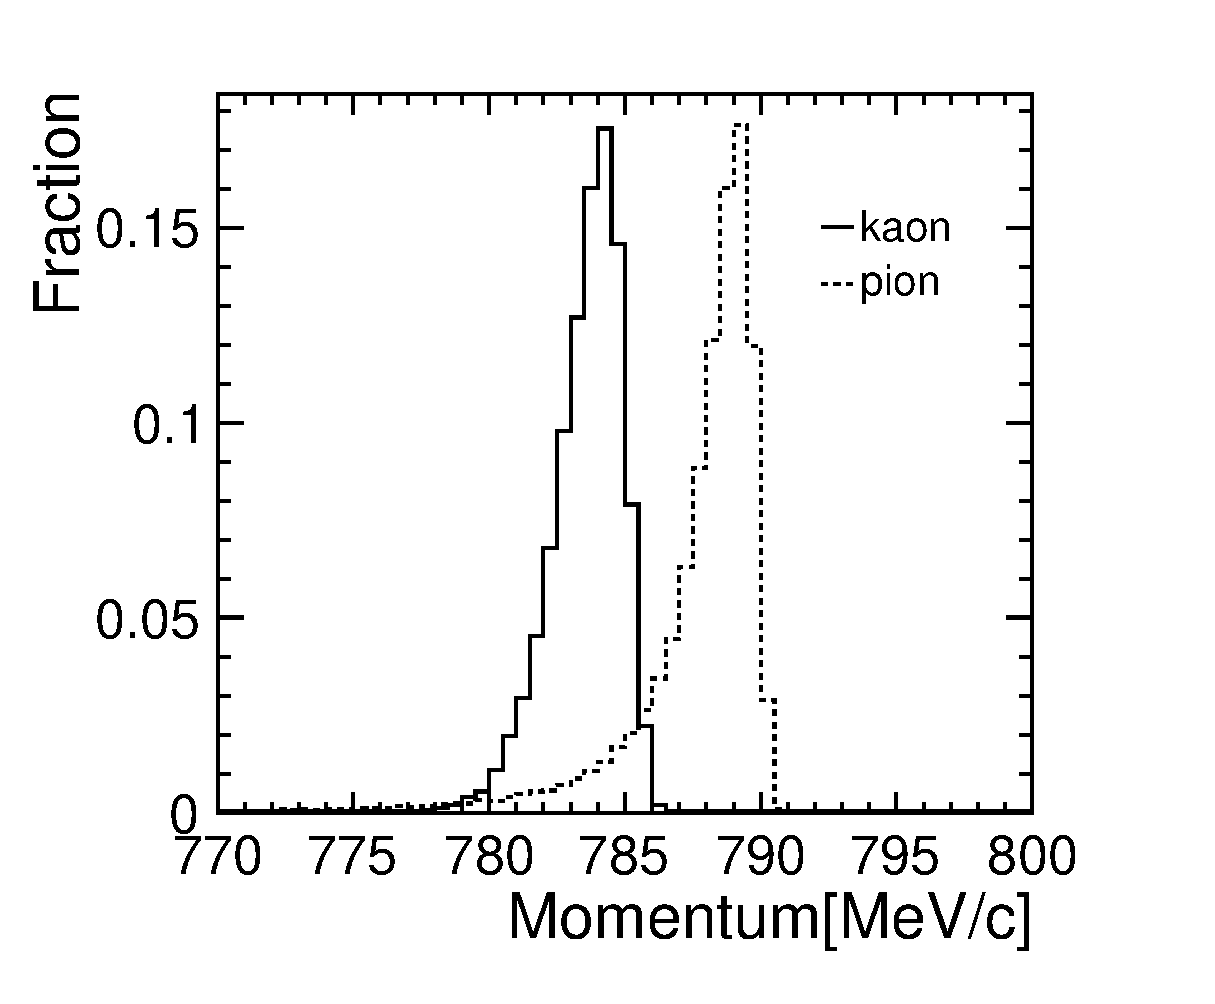
\includegraphics[width=10cm,clip]{./fig/Kaon_pion_momentum_nogrid.eps}
  \caption{Kaon and Pion momentum distribution at BDC}
  \label{k_pi_momentum}
\end{figure}


\subsubsection{Kaon energy
  \label{KaonEnergy}
}
Kaon beam momentum is estimated by the momentum distribution of MC simulation.
We change Kaon beam momentum in a range of 700 - 800 MeV/$c$ and search the momentum that decay point distribution of MC simulation is consistent with data one.

\subsubsection{Proton energy}
Proton momentum shown in Figure \ref{fig:Proton_momentum} is used as proton beam momentum of MC simulation.

\subsubsection{Energy deposition in degrader}
It is too high energy that Kaon beam stops in the fiducial volume of 250LAr TPC.
In order to degrade the beam momentum, some lead glass blocks and a lead brick were inserted in front of 250LAr TPC as degrader.
%We estimate energy deposition in degrader by using MC simulation.
Figure \ref{energy_deposition} shows energy deposition distribution in degrader.


\begin{figure}[!htb]
  \centering
  \centering
  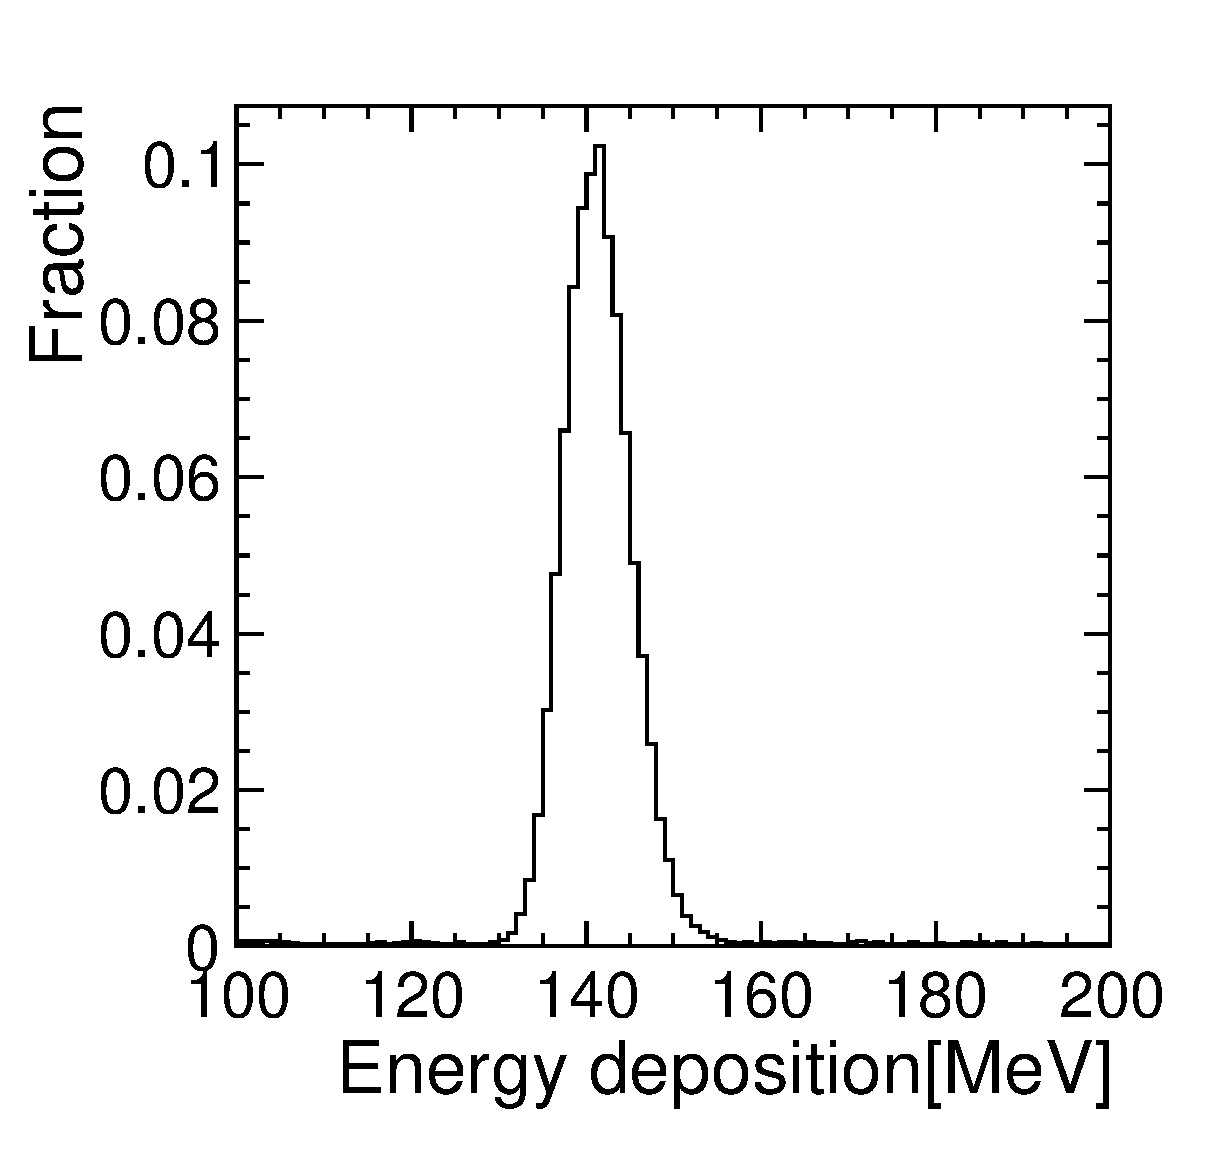
\includegraphics[width=10cm,clip]{./fig/energy_deposition.eps}
  \caption{Energy deposition in degrader}
  \label{energy_deposition}
\end{figure}






%%%%%%%%%%%%%%%%%%%%%%%%%%%%%%%%%%%%%%%%%%%%%%%%%%
%\section{Pion Result}
%%%%%%%%%%%%%%%%%%%%%%%%%%%%%%%%%%%%%%%%%%%%%%%%%%
\section{Through-going Pion}
\label{Sec:Pion}
\begin{itemize}
\item Explain Landau distribution ("bare" track and "dressed" track)
\item pion track (800 MeV/c) and soft electron ($\sim$10 keV) has different $dE/dx$ = recombination
\item Set delta-ray cut off = 10 keV in simulation, and take ICARUS measurement of recombination.
\item Hit charge distribution is in good agreement between data and MC.
\end{itemize}

\begin{figure}[htbp]
 \begin{center}
  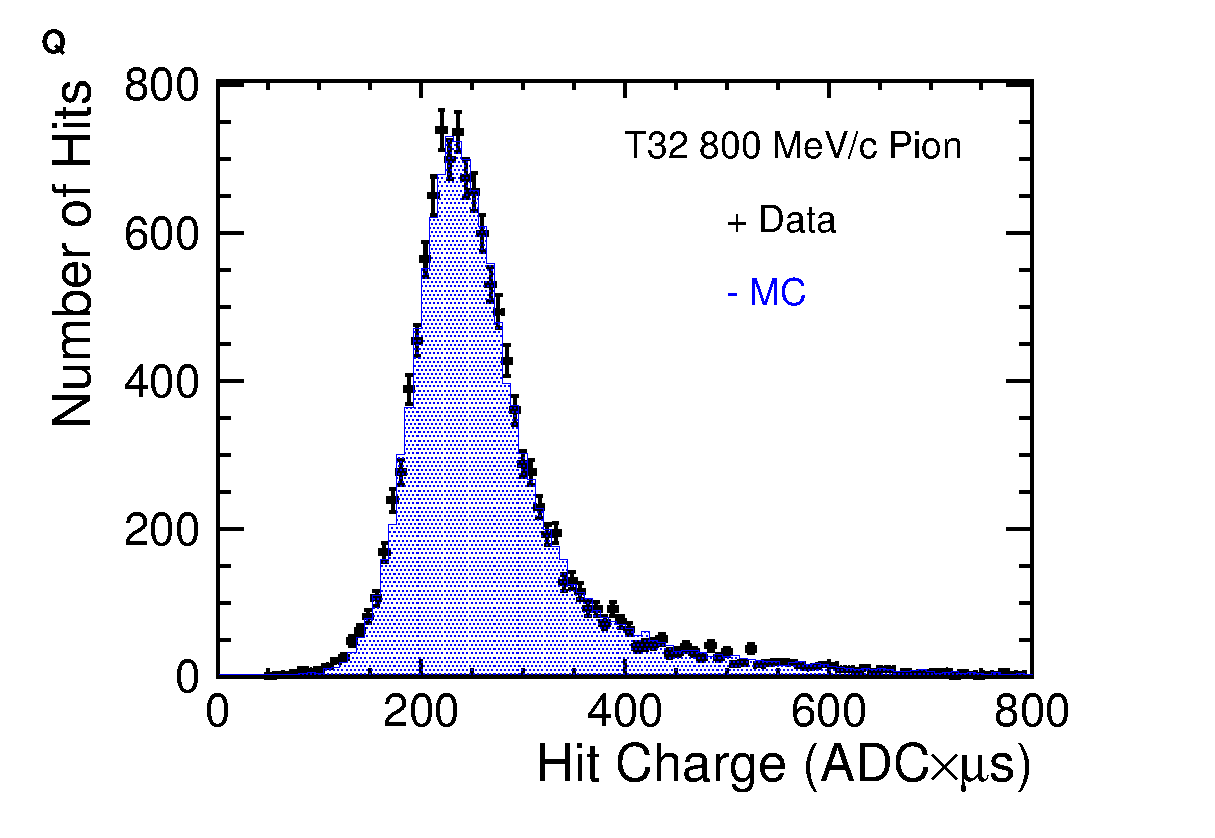
\includegraphics[width=0.8\hsize]{fig/PionLandau.eps}
 \end{center}
 \caption{Hit charge distribution for 800 MeV/c through-going $\pi^+$ sample. Points and histograms correspond to data and MC, respectively}
 \label{Fig:PionLandau}
\end{figure}

%%%%%%%%%%%%%%%%%%%%%%%%%%%%%%%%%%%%%%%%%%%%%%%%%%
%\section{Proton Result}
%%%%%%%%%%%%%%%%%%%%%%%%%%%%%%%%%%%%%%%%%%%%%%%%%%
\section{Stopped Proton}
\label{Sec:Proton}

%
%Proton events are applied following simple selections.
Proton event selection
\begin{itemize}
\item Protons are selected by the information of beam counters.
\item Drift time of the hit at the injection point: 150$mu$s to 300$\mu$s which corresponds with T32 BDC fiducial volume.
\item Total number of hits in the cluster is greater than 5.
%\item Only one hit are required at the same channel in the cluster to remove multi-track events.
\item Only one cluster in the event
\end{itemize}

For good proton events, we compare each parameter between data and MC.
Figure\ref{fig:various_distribution} shows the comparison of the distribution of 
Hit Charge, Hit Sigma, Stopped Channel and  Cluster Charge between data and MC.
All four distributions of MC reproduce data well.
Especially, the agreement of stopped channel distribution shows the consistent 
the momentum estimation by TOF information with the initial momentum of the particles injected to 250L detector.\\

\begin{figure}[htbp]
  \centering
  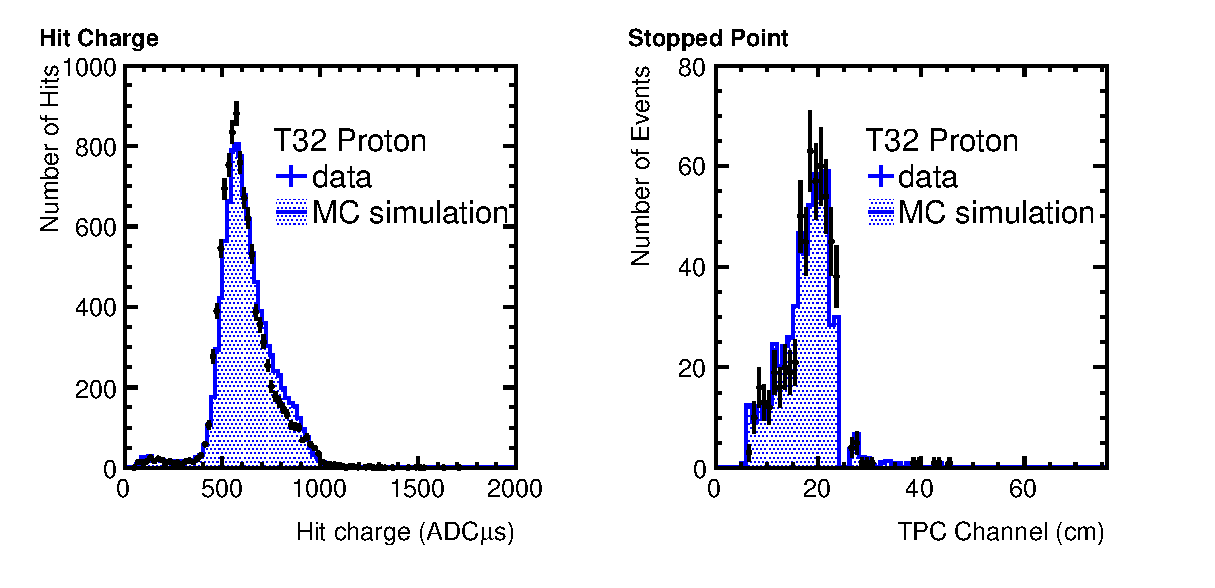
\includegraphics[width=1.0\hsize,clip]{./fig/Proton_1.eps}
  \caption{Hit Charge, Hit Sigma, Stopped Channel, Cluster Charge}
  \label{fig:various_distribution}
\end{figure}

Figure\ref{fig:ADC_distribution} shows the hit charge distribution of each distance from stopped point.
Hit charge distributions of MC simulation are good agreements with data.
Figure\ref{fig:Mean_comparison} shows the mean of the hit charge distribution of each distance from stopped point.
%Figure\ref{fig:Mean_comparison_ratio} shows the ratios of Data/MC.
%The ratios are within 94\%$\sim$105\%.
MC simulation reproduce the charge response of data in high and wide dE/dx region well.

\begin{figure}[htbp]
  \centering
  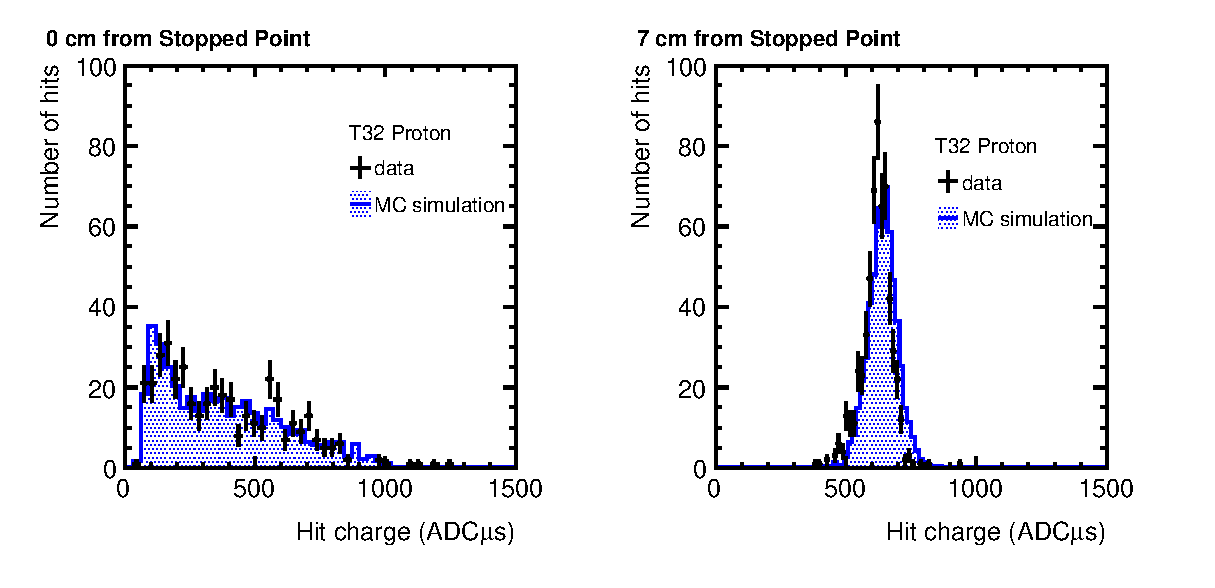
\includegraphics[width=1.0\hsize,clip]{fig/Proton_2.eps}
  \caption{Hit charge distribution of each distance from stopped point}
  \label{fig:ADC_distribution}
\end{figure}

%\begin{figure}[htbp]
%  \begin{center}
%  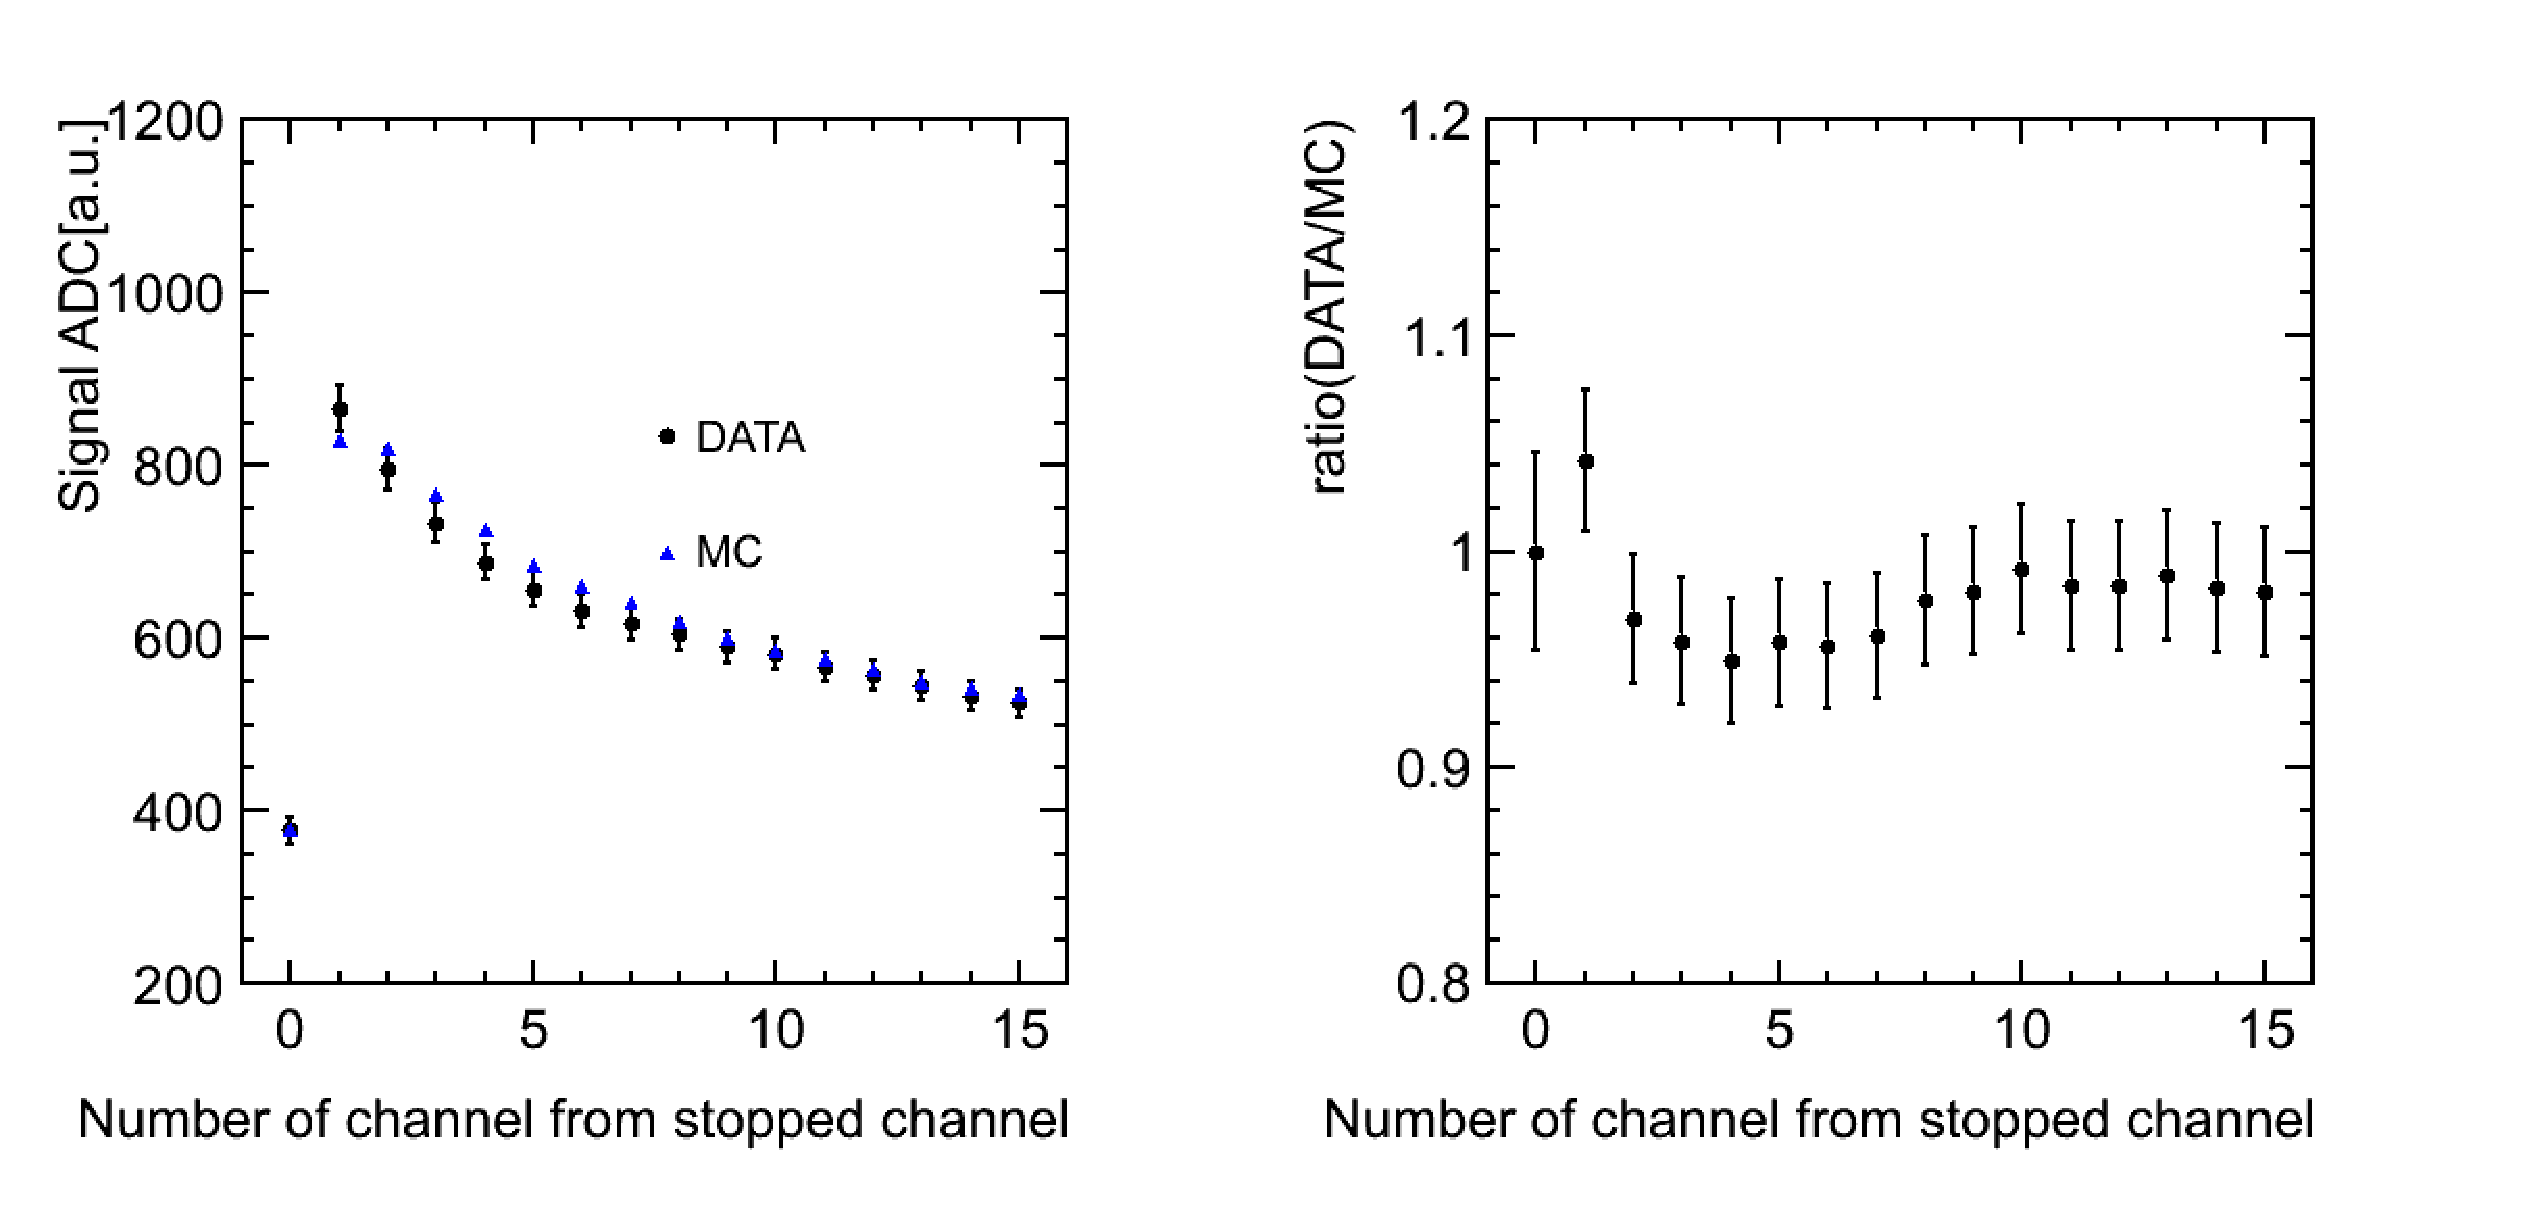
\includegraphics[width=1.0\hsize,clip]{fig/stop_proton3.eps}
%  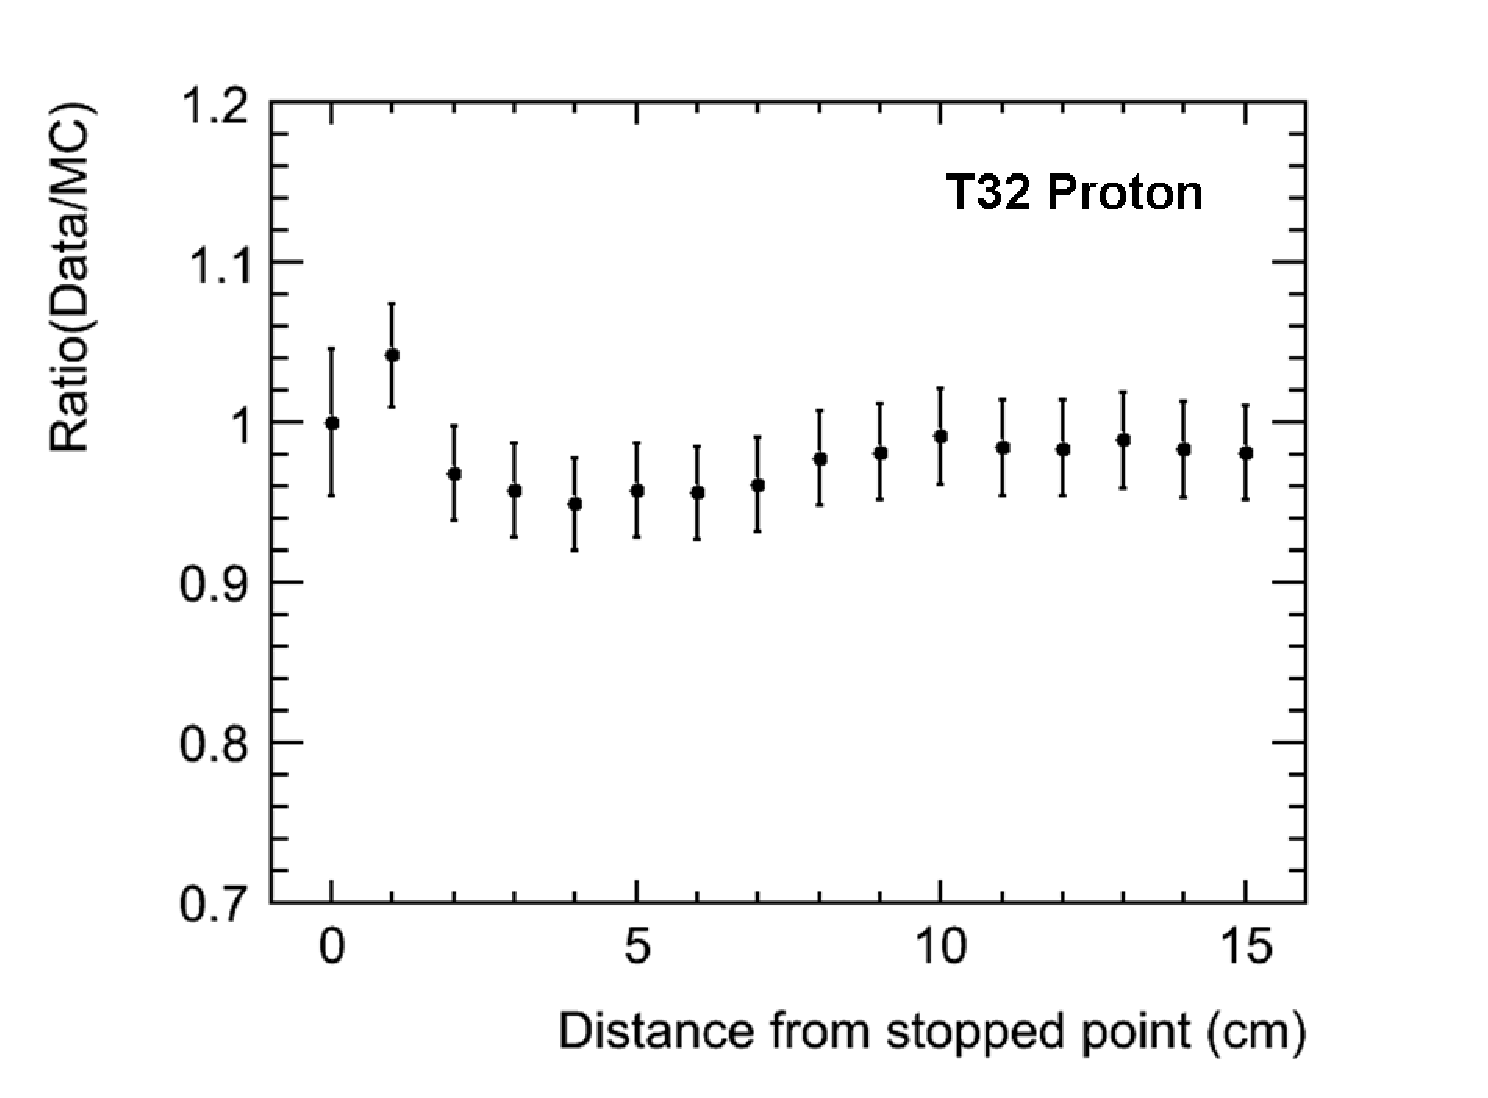
\includegraphics[width=0.8\hsize,clip]{fig/stop_proton4.eps}
%  \end{center}
%  \caption{Data-MC comparison of the mean of hit charge distribution}
%  \label{fig:Mean_comparison}
%  \label{fig:Mean_comparison_ratio}
%\end{figure}

% LocalWords:  fiducial


\subsection{Recombination Factor}

For the data-MC comparison, we use parameters of the recombination factor in ICARUS measurement of Ref.\cite{658352}.
In this section, we measure the recombination factor using proton (and Kaon) data.

% Electron-ion recombination depends on the electric field and stopping power $dE/dx$. We study this factor using tagged proton beam. 
%Recombination factor measurement using proton beam is relatively easy because of stability of proton. 
%This is why we used proton beam for this study as a first step.\\

  Expression for recombination (Birks law) in Eq.~\ref{eq:birkslaw} can can be rearranged like below:
\begin{equation}
  \frac{Q_{0}}{Q} = \frac{1}{A}+\frac{(k/E)(dE/dx)(1/\rho)}{A}
\end{equation}

In this equation, the ratio of $Q_{0}/Q$ has linear dependence of stopping power $dE/dx$,
and $Q$ from data (See Fig.~\ref{fig:Mean_comparison}), $Q_{0}$ and $dE/dx$ from MC can be determined for every distance from the stopped point.
By using this we are able to extract parameters $A$ and $k$.
$Q_{0}$ is determined from the simulation sample without recombination (Top left plot in Fig.~\ref{Fig:Preco}), and $dE/dx$ per an anode channel is determined with truth information of simulation (Top right plot in Fig.~\ref{Fig:Preco}). 
The result of this study is shown in bottom plot of Fig\ref{Fig:Preco}. Vertical axis is $Q_{0}/Q$, and horizontal axis is $dE/dx$ in this figure, this plot is fitted to straight line.
As a result, we obtain fitting parameter, $A$ = 0.832$\pm$0.009(stat.)$\pm$0.006(syst.), and $k$=0.0504$\pm$0.0010(stat.)$\pm$0.0013(syst.) [kV(g/cm$^{2}$)/cm/MeV]

It confirms Birks law in the range of 4  $\leqq$ dE/dx $\leqq$ 12 MeV/$cm^2$ and electric field of 200 V/cm is consistent with ICARUS measurement\cite{658352}.
 $A$ = 0.800$\pm$0.003 and $k$=0.0486$\pm$0.0006 [kV(g/cm$^{2}$)/cm/MeV]

%ch by ch data distribution
%\begin{figure}[!htb]
%  \begin{center}
%  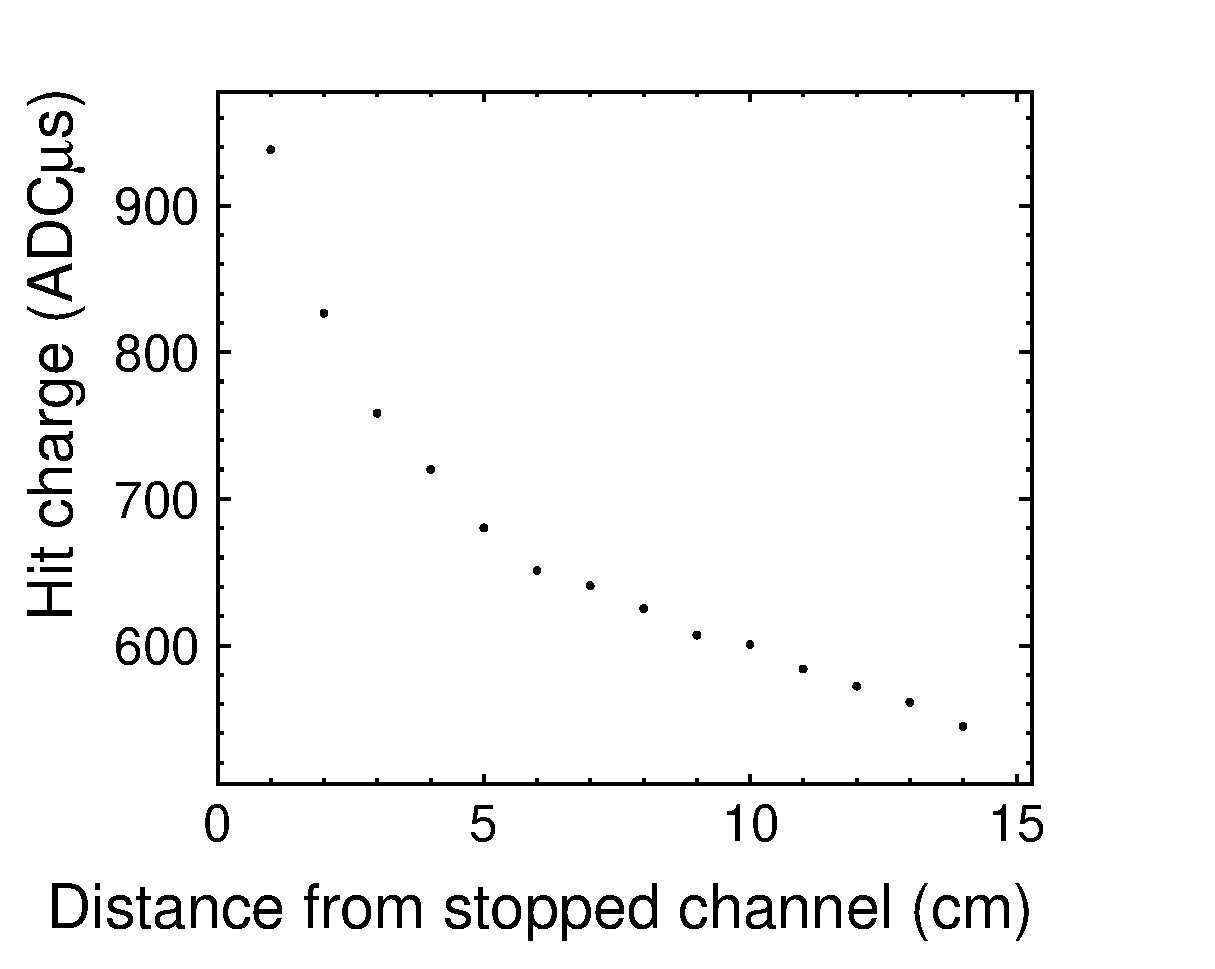
\includegraphics[0.3\hsize,clip]{./fig/Q2.eps}
%  \includegraphics[width=11cm,clip]{./fig/Data_FADCdistChbyCh.eps}
%  \caption{DATA:Integrated Flash ADC counts from stopped channel -1}
%  \label{fadcDist1}
%\end{figure}
%
%ch by ch MC distribution
\begin{figure}[!htb]
  \begin{center}
%    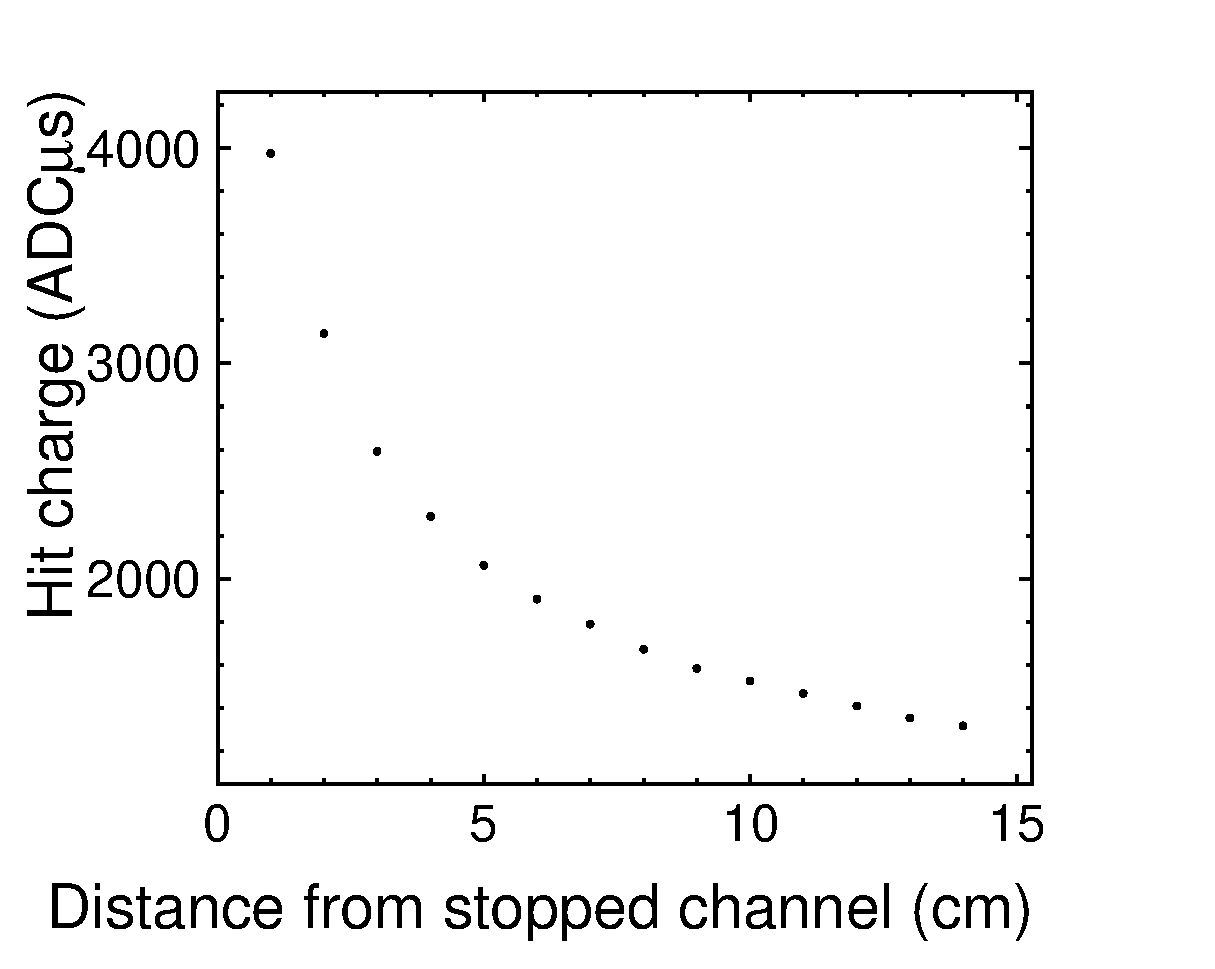
\includegraphics[width=0.45\hsize,clip]{./fig/Q_02.eps}
%    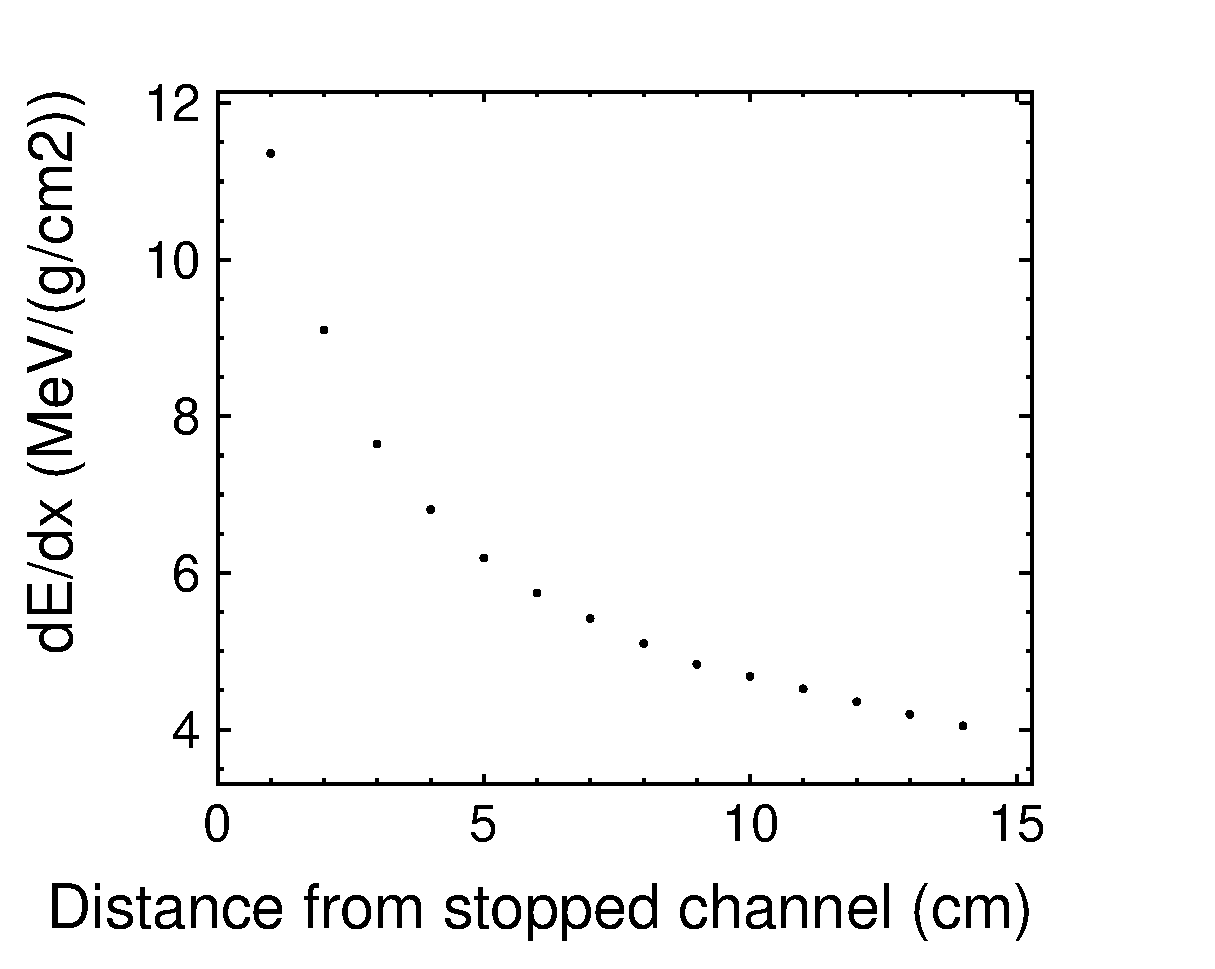
\includegraphics[width=0.45\hsize,clip]{./fig/dEdx2.eps}
    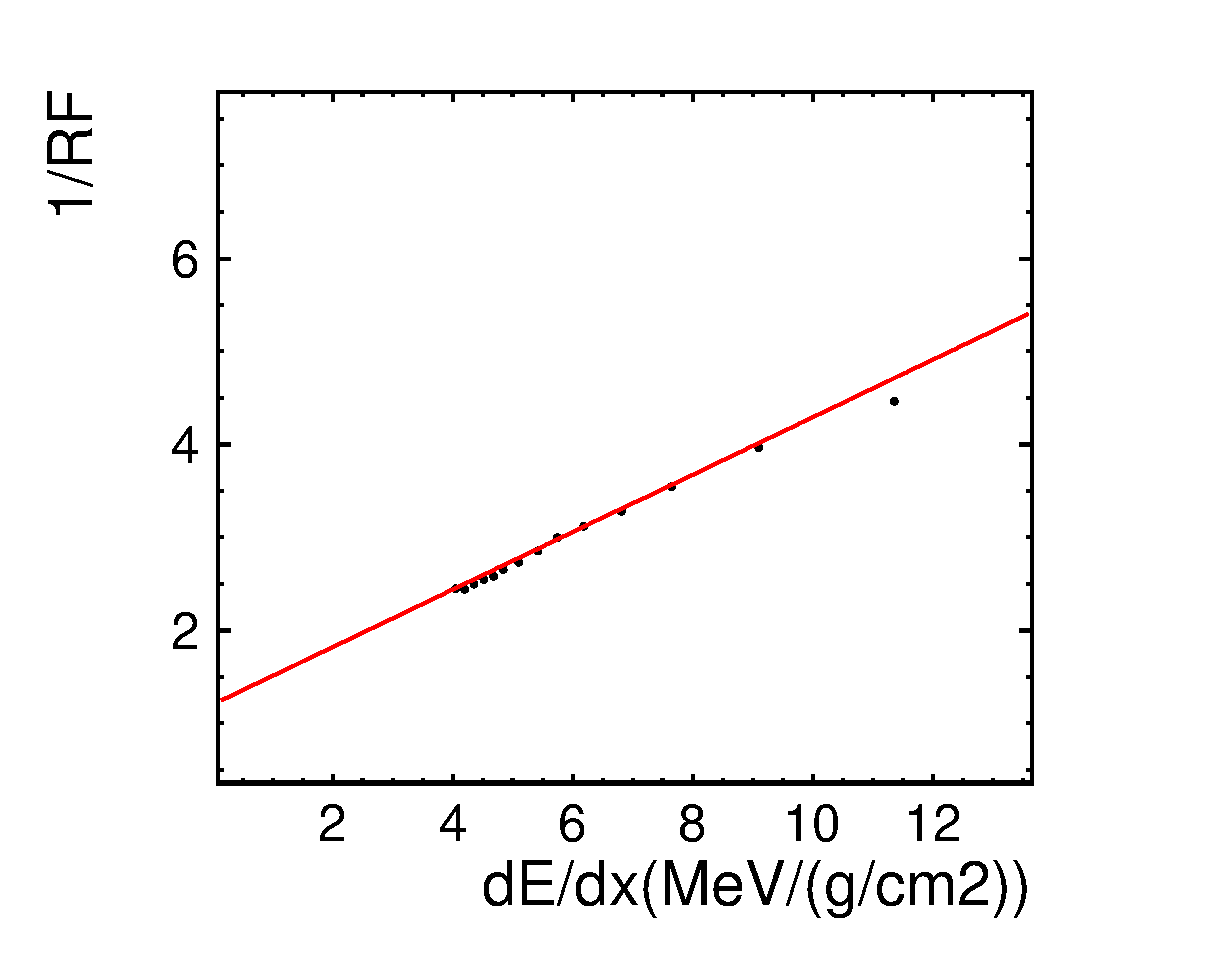
\includegraphics[width=0.8\hsize,clip]{./fig/RFresult2.eps}
%    \caption{Top left and top right plots show simulated hit charge without recombination ($Q_0$) and
%      average energy deposition ($dE/dx$) respectively as a function of the distance from the proton stopped point,
%      and bottom plot shows 1/RF VS dE/dx fitted by Birks law}
    \caption{$Q_0/Q$ as a function of $dE/dx$ fitted to linear line to extract parameters of Birks law}
    %  \caption{Distribution of dE/dx ch by ch}
    %  \caption{dE/dx from stopped channel -1}
    \label{Fig:Preco}
  \end{center}
\end{figure}
%
%result

%\begin{figure}[!htb]
%  \centering
%  \centering
%  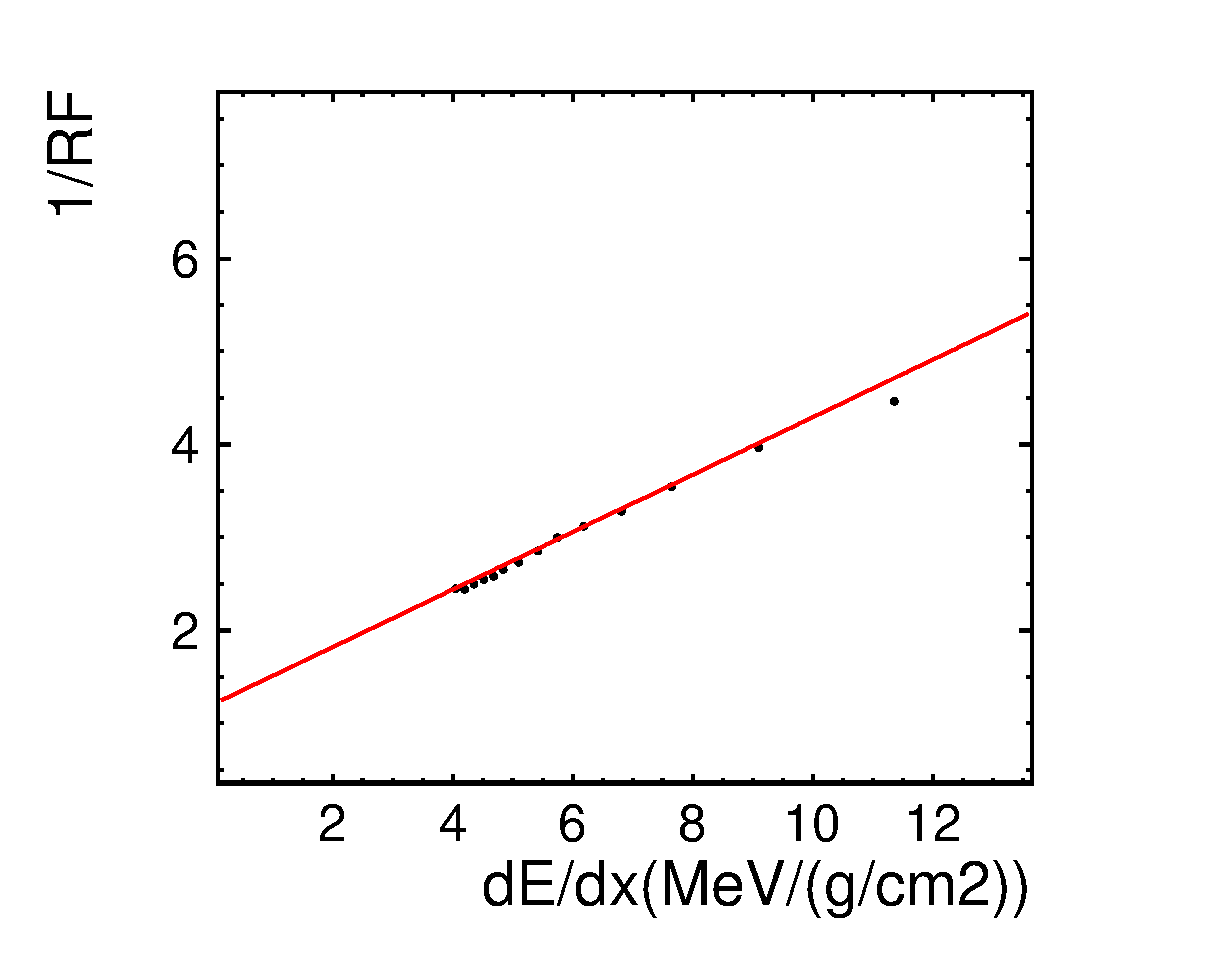
\includegraphics[width=0.8\hsize,clip]{./fig/RFresult2.eps}
%  \caption{1/RF VS dE/dx: fitted by Birks law}
%  \label{result}
%\end{figure}

%%%%%%%%%%%%%%%%%%%%%%%%%%%%%%%%%%%%%%%%%%%%%%%%%%
%\section{Kaon Result}
%%%%%%%%%%%%%%%%%%%%%%%%%%%%%%%%%%%%%%%%%%%%%%%%%%
\subsection{Stopped Kaon}
\label{Sec:Kaon}
\begin{itemize}
\item Stopping point of the Kaon is identified as kink of the track
\item For example, $K\to\mu\nu$ event (Fig.~\ref{Fig:SimulatedKaon}) is composed by two tracks, Kaon and muon, and intersection of two tracks corresponds to the stopped point.
\item We develop two different algorithm to identify the Kaon stopped point, Hough and Chi2.
\end{itemize}

Hough transform was invented for machine analysis of bubble chamber photographs by Paul.V.C.Hough.\cite{3069654}.
\begin{itemize}
\item Transform hit coordinates [TPC channel, drift time] into Hough space
\item Find the straight line by choosing the most dense point in Hough space (= Kaon track)
\item Hits associated with the first straight line are removed, and remaining hit coordinates are transformed into Hough space.
\item Find second straight line using the same procedure ( = Muon track)
\item This procedure is repeated until number of remaining hits are less than three.
\item Kaon stopped point is identified as the hit with maximum charge and around the intersection of two lines.
\end{itemize}

%Figure \ref{hmap2} shows hit map like a Kaon track.
%One point in the X-Y space can be transformed into sinusoidal curve in the $\rho$-$\theta$ space.Figure \ref{rho_theta2} shows sinusoidal curves in all points.
%And, we find the straight line associated with the largest number of points by choosing the most dense point in $\rho$-$\theta$ space.
%Next , the sinusoidal curves of the hits associated with frist straight line are removed from figure \ref{rho_theta2}.
%Figure \ref{rho_theta3} shows sinusoidal curves after the hits associated with frist straight line removed.
%We find second straight line using the same procedure.This procedure is repeated until there are less than three points.
%Figure \ref{hmap_fit} shows the two straight lines found by hough transform mehotd.\\
%Kaon stopped point in the liquid argon detecor defined as charge maximum point around the intersection of some lines.

%\begin{figure}[!htb]
%  \begin{minipage}{0.5\hsize}
%    \begin{center}
%      \includegraphics[width=35mm]{fig/hmap2.eps}
%    \end{center}
%    \caption{Hit map like a Kaon track}
%    \label{hmap2}
%  \end{minipage}
%  \begin{minipage}{0.5\hsize}
%    \begin{center}
%      \includegraphics[width=35mm]{fig/rho_theta2.eps}
%    \end{center}
%    \caption{sinusoidal curves getting form all hough transformed  points of Figure \ref{hmap2}}
%    \label{rho_theta2}
%  \end{minipage}
%  \\
%  \begin{minipage}{0.5\hsize}
%    \begin{center}
%      \includegraphics[width=35mm]{fig/rho_theta_kink.eps}
%    \end{center}
%    \caption{sinusoidal curves removed the points associated with first straight line from figure \ref{rho_theta2}}
%    \label{rho_theta3}
%  \end{minipage}
%  \begin{minipage}{0.5\hsize}
%    \begin{center}
%      \includegraphics[width=35mm]{fig/hmap_fit.eps}
%    \end{center}
%    \caption{Two lines found with hough transform method}
%    \label{hmap_fit}
%  \end{minipage}
%\end{figure}


%\subsubsection{Chi2 method}

$\chi^{2}$ method is the algorithm to 
Identify the kaon stopped point as  the point which rapidly increase fit $\chi^{2}$ to straight line.
\begin{itemize}
\item Starting from the most upstream hit in the cluster, fit the hits to straight line (Kaon track)
\item Find the point which rapidly increase fit $\chi^{2}$ to straight line.
\item Starting from the most downstream hit in the cluster, fit the hits to straight line (Muon track)
\item Find the point which rapidly increase fit $\chi^{2}$ to straight line.
\item Kaon stopped point is identified as the hit with maximum charge and around the intersection of the two lines.
\end{itemize}

Figure \ref{KsomeQuantities} shows Data and MC comparison for signal hit charge, signal width, decay point and total particle charge distribution.
Data of signal charge and signal width are consistent with MC one in error by less than two $\%$ and data of cluster charge and primary charge are consistent with  
MC one in error by less than five $\%$.

%Figure \ref{cq27_hough} shows signal hit charge distribution of restricted channel 27. 
%As shown in figure \ref{cq27_hough}, signal charge have two peaks at 300 and 500 ADCus.
%Because two peaks has correlation of $\Delta$TOF, possible assumption of the cause is that beam line were bipolarrized and the beam didn't pass in the center of the detector.
%So, we use only the event that signal charge of restricted channel 27 is less than 350.
%Figure \ref{RangeVsHit_hough} shows signal hit charge distribution in different distance from the stopped point.

\begin{figure}[htbp]
  \begin{center}
    \includegraphics[width=1.0\hsize]{fig/cHit4_hough.eps}
  \end{center}    
    \caption{Data-MC comparison for hit charge, hit sigma, cluster charge, primary particle charge}
    \label{KsomeQuantities}
\end{figure}

%\begin{figure}[!htb]
%  \begin{center}
%    \includegraphics[width=70mm]{fig/ch27distribution.eps}
%  \end{center}
%  \label{cq27_hough}
%  \caption{Hit charge in channel 27}
%\end{figure}

%\begin{figure}[!htb]
%  \begin{center}
%    \includegraphics[width=0.8\hsize]{fig/RangeVsHit4_wcut_hough.eps}
%  \end{center}
%  \caption{Data-MC comparison for hit charge distribution in different distance from the stopped point(top left:decay point,top light:decay point-5cm,bottom left:decay point-10cm,decay point-15cm)}
%  \label{RangeVsHit_hough}
%\end{figure}

%As shown in figure \ref{RangeVsHit_hough}, data is consistent with MC one.
Figure \ref{RangeVsHitRatio_hough} shows data/MC ratio of signal hit charge distribution in different distance from the stopped point.
Data of signal charge in different distance from stopped point are consistent with MC one with in 5$\%$.

\begin{figure}[htb]
  \begin{center}
    \includegraphics[width=1.0\hsize]{fig/RangeVsHitfabs_wcut_hough.eps}
 %   \includegraphics[width=0.8\hsize]{fig/RangeVsHitRatio_wcut_hough.eps}
  \end{center}
  \caption{Top plot shows Data-MC comparison for hit charge distribution in different distance from the stopped point.
    Bottom plot shows Data/MC ratio for hit charge distribution in different distance from the stopped point}
  \label{RangeVsHitfabs_hough}
  \label{RangeVsHitRatio_hough}
\end{figure}




%%%%%%%%%%%%%%%%%%%%%%%%%%%%%%%%%%%%%%%%%%%%%%%%%%%
%\section{Recombination Factor}
%%%%%%%%%%%%%%%%%%%%%%%%%%%%%%%%%%%%%%%%%%%%%%%%%%
%\subsection{Recombination Factor}

For the data-MC comparison, we use parameters of the recombination factor in ICARUS measurement of Ref.\cite{658352}.
In this section, we measure the recombination factor using proton (and Kaon) data.

% Electron-ion recombination depends on the electric field and stopping power $dE/dx$. We study this factor using tagged proton beam. 
%Recombination factor measurement using proton beam is relatively easy because of stability of proton. 
%This is why we used proton beam for this study as a first step.\\

  Expression for recombination (Birks law) in Eq.~\ref{eq:birkslaw} can can be rearranged like below:
\begin{equation}
  \frac{Q_{0}}{Q} = \frac{1}{A}+\frac{(k/E)(dE/dx)(1/\rho)}{A}
\end{equation}

In this equation, the ratio of $Q_{0}/Q$ has linear dependence of stopping power $dE/dx$,
and $Q$ from data (See Fig.~\ref{fig:Mean_comparison}), $Q_{0}$ and $dE/dx$ from MC can be determined for every distance from the stopped point.
By using this we are able to extract parameters $A$ and $k$.
$Q_{0}$ is determined from the simulation sample without recombination (Top left plot in Fig.~\ref{Fig:Preco}), and $dE/dx$ per an anode channel is determined with truth information of simulation (Top right plot in Fig.~\ref{Fig:Preco}). 
The result of this study is shown in bottom plot of Fig\ref{Fig:Preco}. Vertical axis is $Q_{0}/Q$, and horizontal axis is $dE/dx$ in this figure, this plot is fitted to straight line.
As a result, we obtain fitting parameter, $A$ = 0.832$\pm$0.009(stat.)$\pm$0.006(syst.), and $k$=0.0504$\pm$0.0010(stat.)$\pm$0.0013(syst.) [kV(g/cm$^{2}$)/cm/MeV]

It confirms Birks law in the range of 4  $\leqq$ dE/dx $\leqq$ 12 MeV/$cm^2$ and electric field of 200 V/cm is consistent with ICARUS measurement\cite{658352}.
 $A$ = 0.800$\pm$0.003 and $k$=0.0486$\pm$0.0006 [kV(g/cm$^{2}$)/cm/MeV]

%ch by ch data distribution
%\begin{figure}[!htb]
%  \begin{center}
%  \includegraphics[0.3\hsize,clip]{./fig/Q2.eps}
%  \includegraphics[width=11cm,clip]{./fig/Data_FADCdistChbyCh.eps}
%  \caption{DATA:Integrated Flash ADC counts from stopped channel -1}
%  \label{fadcDist1}
%\end{figure}
%
%ch by ch MC distribution
\begin{figure}[!htb]
  \begin{center}
%    \includegraphics[width=0.45\hsize,clip]{./fig/Q_02.eps}
%    \includegraphics[width=0.45\hsize,clip]{./fig/dEdx2.eps}
    \includegraphics[width=0.8\hsize,clip]{./fig/RFresult2.eps}
%    \caption{Top left and top right plots show simulated hit charge without recombination ($Q_0$) and
%      average energy deposition ($dE/dx$) respectively as a function of the distance from the proton stopped point,
%      and bottom plot shows 1/RF VS dE/dx fitted by Birks law}
    \caption{$Q_0/Q$ as a function of $dE/dx$ fitted to linear line to extract parameters of Birks law}
    %  \caption{Distribution of dE/dx ch by ch}
    %  \caption{dE/dx from stopped channel -1}
    \label{Fig:Preco}
  \end{center}
\end{figure}
%
%result

%\begin{figure}[!htb]
%  \centering
%  \centering
%  \includegraphics[width=0.8\hsize,clip]{./fig/RFresult2.eps}
%  \caption{1/RF VS dE/dx: fitted by Birks law}
%  \label{result}
%\end{figure}

%%%%%%%%%%%%%%%%%%%%%%%%%%%%%%%%%%%%%%%%%%%%%%%%%%
%\section{Summary}
%%%%%%%%%%%%%%%%%%%%%%%%%%%%%%%%%%%%%%%%%%%%%%%%%%
\section{Summary}
\begin{itemize}
\item We have constructed 250L LArTPC
\item Collected high purity Pion, Kaon, and proton sample
\item Establish Kaon stopped point finding algorithm
\item Develop realistic detector simulation
\item Good understanding of Pion Landau distribution
\item Good understanding of Proton and Kaon dE/dx
\item Measurement of recombination using pi, K, and proton
\end{itemize}


%% The Appendices part is started with the command \appendix;
%% appendix sections are then done as normal sections
%% \appendix

%% \section{}
%% \label{}

%% References
%%
%% Following citation commands can be used in the body text:
%% Usage of \cite is as follows:
%%   \cite{key}         ==>>  [#]
%%   \cite[chap. 2]{key} ==>> [#, chap. 2]
%%

%% References with bibTeX database:

\bibliographystyle{elsarticle-num}
\bibliography{<your-bib-database>}

%% Authors are advised to submit their bibtex database files. They are
%% requested to list a bibtex style file in the manuscript if they do
%% not want to use elsarticle-num.bst.

%% References without bibTeX database:

\begin{thebibliography}{00}

%% \bibitem must have the following form:
%%   \bibitem{key}...
%%

% \bibitem{}
%\cite{Araoka:2011pw}
\bibitem{Araoka:2011pw}
  O.~Araoka {\it et al.},
  %``A tagged low-momentum kaon test-beam exposure with a 250L LAr TPC (J-PARC
  %T32),''
  J.\ Phys.\ Conf.\ Ser.\  {\bf 308}, 012008 (2011)
  [arXiv:1105.5818 [physics.ins-det]].
  %%CITATION = 00462,308,012008;%%

\bibitem{Mihara:2004ft}
S.~Mihara [MEG Collaboration],
%``R&D work on a liquid-xenon photon detector for MEG experiment at PSI,''
Nucl.\ Instrum.\ Meth.\ A {\bf 518}, 45 (2004).
%%CITATION = NUIMA,A518,45;%%

%\cite{658352}
\bibitem{658352} 
  S.~Amoruso {\it et al.} [ICARUS Collaboration],
  %``Study of electron recombination in liquid argon with the ICARUS TPC,''
  Nucl.\ Instrum.\ Meth.\ A\ {\bf 523}, 275  (2004).
  %%CITATION = NUIMA,A523,275;%%

%\cite{649233}
\bibitem{649233} 
  S.~Amoruso, M.~Antonello, P.~Aprili, F.~Arneodo, A.~Badertscher, B.~Baibusinov, M.~Baldo-Ceolin and G.~Battistoni {\it et al.},
  %``Analysis of the liquid argon purity in the ICARUS T600 TPC,''
  Nucl.\ Instrum.\ Meth.\ A\ {\bf 516}, 68  (2004).
  %%CITATION = NUIMA,A516,68;%%

\bibitem{purity}
  A.~Bettini {\it et al.}, Nucl.\ Instrum.\ Meth.\ A\ {\bf 305}, 177 (1991).

\bibitem{Ref:FEMTET}
http://www.muratasoftware.com/products/index.html

\bibitem{3069654}
  P.V.C Hough 'Method and means for recognizing complex patterns',United States Patent Office 3069654(1962) 

\end{thebibliography}


\end{document}

%%
%% End of file `elsarticle-template-num.tex'.
